% =====================================================================
% competition-statement-template.tex
% 通用参赛作品说明书 LaTeX 模板（ distilled framework ）
%
% 设计原则：
%   1. 基础类用 harryopo-report.cls（自带封面+摘要+目录+章节+页眉页脚）
%   2. 章节结构支持 6+1 模式，保留 1.1/2.1/2.2.1 多级编号
%   3. 图片位置提前预留，用户只需把图片拖入 figures/ 即可
%   4. 表格占位用 tabularx 自适应列宽，标题标注"内容类型"
%   5. 风格蒸馏：方正文宋系 + 强数据感 + 第一人称叙述
%   6. 通用化：支持 AI 软件 / 硬件 / 社会创新三类项目
%
% 使用流程：
%   a) 双击 build.bat 或运行 ./build.ps1 编译（自动 3 遍 xelatex）
%   b) 把图片命名为约定格式后拖入 figures/ 目录
%   c) 替换正文{占位}文字为你自己的内容
%   d) 重新编译即出新 PDF
% =====================================================================

% =====================================================================
% 配置区（用户按项目类型修改此处即可）
% =====================================================================
% 项目类型：AISOFTWARE / HARDWARE / SOCIAL
%   AISOFTWARE - AI/软件/互联网项目（默认）
%   HARDWARE   - 硬件/嵌入式/机器人项目
%   SOCIAL     - 社会创新/设计/文创项目
\newcommand{\projectType}{AISOFTWARE}

% 评审标准维度（4 行，按比赛要求修改）
% 格式：维度名 & 权重 & 评委关心点
\newcommand{\reviewDims}{%
    创新性与创意度 & 20\% & 为什么是这个项目？差异化定位 \\%
    技术实现与复杂度 & 30\% & 它是怎么跑起来的？关键工程指标 \\%
    实用价值与落地性 & 30\% & 它好用吗？真实使用数据 \\%
    用户体验与交互设计 & 20\% & 用起来顺手吗？设计亮点 \\%
}

% 可选章节开关（\xxxfalse 即关闭该章节）
\newif\ifshowteam        \showteamtrue       % 团队介绍
\newif\ifshowexecsummary  \showexecsummarytrue % 一页纸 Executive Summary
\newif\ifshowbib          \showbibtrue         % 参考文献
\newif\ifshowfaq          \showfaqtrue         % FAQ
\newif\ifshowappendix     \showappendixtrue    % 附录（数据合规/使用教程）
\newif\ifshowtools        \showtoolstrue       % 第3章：工具使用与经验总结
\newif\ifshowthoughts     \showthoughtstrue    % 第3章：个人想法
\newif\ifshowcompetitors  \showcompetitorstrue % 第3章：与竞品的差异化
\newif\ifshowreviewdetail \showreviewdetailtrue% 第3章：评审标准对标（详细）
\newif\ifshowvalue        \showvaluetrue       % 第3章：应用价值
\newif\ifshowfuture       \showfuturetrue      % 第3章：未来规划

% =====================================================================
% 摘要模板库（按 \projectType 自动切换）
% =====================================================================
% AI/SOFTWARE 项目摘要模板
\newcommand{\abstractAISoftware}{%
{摘要占位}建议 300-500 字，覆盖 4 块：
(1) 一句话定位（是什么 + 面向谁）
(2) 解决的核心痛点（读了就忘、笔记散乱、想问无门、知道做不到）
(3) 核心创新（方法论自动注入 / 5 维 ContextBuilder / FSRS v5 / 本地优先架构 / ECDICT 离线词典）
(4) 量化成果（数据规模、测试用例、用户使用时长等）
}

% HARDWARE 项目摘要模板
\newcommand{\abstractHardware}{%
{摘要占位}建议 300-500 字，覆盖 4 块：
(1) 一句话定位（是什么 + 面向谁 + 核心功能）
(2) 解决的实际问题（场景痛点 + 现有方案不足）
(3) 技术方案亮点（传感器/算法/结构/交互的 N 大创新）
(4) 验证结果（实验数据、精度、稳定性、成本控制）
}

% SOCIAL 项目摘要模板
\newcommand{\abstractSocial}{%
{摘要占位}建议 300-500 字，覆盖 4 块：
(1) 一句话定位（社会问题 + 目标人群 + 干预方式）
(2) 问题分析（数据/调研/用户痛点）
(3) 解决方案（设计/服务/产品的 N 大创新点）
(4) 落地成效（覆盖人数、合作方、社会影响力评估）
}

\documentclass[12pt,a4paper,nomath]{harryopo-report}

% --- 图片搜索路径 ---
% build.ps1 从 templates/ 子目录编译（让 fonts/ 相对路径生效），
% 所以图从 templates/ 找 junction 到 ../figures/。同时兼容从 .tex 同级直接编译。
\graphicspath{{figures/}{../figures/}{./}{./figures/}}

% --- 作品信息（顶部元数据，封面用） ---
\title{知行读书——AI 驱动的阅读成长 Agent}
\subtitle{帮每一位读者构建自我成长型系统}
\author{张三\quad 计算机应用技术专业\quad 2025000101}
\institute{示例大学\quad 计算机学院}
\date{2026年7月}

% --- 基金/项目支持（可留空） ---
\fundproject{参赛项目：火山引擎 × Trae 创造力大赛}

\begin{document}

% =====================================================================
% 可选：一页纸 Executive Summary（封面后立即插入）
% =====================================================================
\ifshowexecsummary
\section*{Executive Summary}
\addcontentsline{toc}{section}{Executive Summary}
{执行摘要占位}建议 300-400 字，浓缩版说明书，适合评委快速浏览。
覆盖：(1) 一句话定位 (2) 核心痛点 (3) 解决方案 (4) 创新点 (5) 成果数据。
\fi

% =====================================================================
% 第一部分：封面（\maketitle 自动生成）
% =====================================================================
\maketitle

% =====================================================================
% 第二部分：摘要 + 关键词
% =====================================================================
% 风格提示：摘要 300-500 字，覆盖"是什么 + 解决什么 + 怎么解决 + 创新点"
\begin{abstract}
% 按项目类型自动选择摘要模板
\ifx\projectType AISOFTWARE
\abstractAISoftware
\else\ifx\projectType HARDWARE
\abstractHardware
\else
\abstractSocial
\fi\fi
\end{abstract}

% 关键词：5-7 个，分号分隔
% 蒸馏自原文档风格：黑体加粗
\newcommand{\keywords}[1]{%
    \par\vspace{0.6em}%
    \noindent{\bfseries\fzht\color{DarkColor}关键词：}#1\par%
    \vspace{0.5em}%
}
\keywords{AI 阅读智能体；Agent 编排；间隔重复；本地优先架构；方法论自动注入；微信读书 Skill；Electron}

% =====================================================================
% 第三部分：目录（自动生成，含插图/表格目录）
% =====================================================================
\tableofcontents

% =====================================================================
% 第四部分：引言
% =====================================================================
\introduction
% 风格提示：用第一人称简述项目缘起、研究动机、整篇文档结构
{引言占位}建议 200-300 字，按三段式：
第一段：为什么要做这个项目（真实痛点/灵感来源）
第二段：本说明书要回答评审最关心的几个问题
第三段：文档组织结构（一句话点出 6 章分别讲什么）

% =====================================================================
% 第 1 章：项目概述
% =====================================================================
\chapter{项目概述}

\section{一句话定位}
% 风格提示：30-50 字的"电梯演讲"，覆盖 3 元素（是什么 + 有什么 + 区别性）
{占位}把「微信读书 → Anki 同源科学记忆 → AI Agent」装进一个本地优先的桌面应用，具有 16 大功能模块和 5 大核心创新；面向所有阅读者，帮每一位读者构建起属于自己的自我成长型系统；在同类产品中，首次将微信读书生态同步、FSRS v5 间隔重复算法与教学策略驱动型 AI Agent 三者深度整合。

\section{是什么/解决什么/怎么做}
% 风格提示：用"题目小标题"格式，黑体 11pt，加粗
\subhead{是什么}基于 XXX 生态的 AI 驱动 XXX 智能体（XXX 桌面应用）
\subhead{解决什么}XX、XX、XX、XX 的四大核心痛点
\subhead{怎么做}同步 → 蒸馏 → 复习 → 应用的完整闭环；本地 SQLite 存储 + API 云端调用

\section{评审标准对标概览}
% 风格提示：4-6 行，每行"评审维度 + 评委关心 + 你的答案"
\begin{table}[htbp]
\centering
\begin{tabularx}{\textwidth}{>{\bfseries\color{MainColor}}l X}
\toprule
\textbf{评审维度（权重）} & \textbf{本作品回答} \\
\midrule
\reviewDims
\bottomrule
\end{tabularx}
\caption{评审标准对标概览（详见第 \ref{sec:review} 节）}
\label{tab:review-overview}
\end{table}

% =====================================================================
% 可选：团队介绍
% =====================================================================
\ifshowteam
\section{团队介绍}
{占位}介绍团队背景、成员分工、协作模式。可配团队合照或分工表。
\fi

% =====================================================================
% 第 2 章：详细介绍
% =====================================================================
\chapter{详细介绍}

\section{解决的问题}
% 风格提示：先 1 段引出"现有工具链是断裂的"，再用 7-8 行表格对照痛点/现状/方案
{引文占位}信息爆炸时代，人们读得越来越多，记住的越来越少。现有工具链是断裂的：阅读在一个 App，笔记在另一个 App，复习又在一个 App，AI 问答更像是完全独立的 ChatGPT 副本。

\begin{table}[htbp]
\centering
\begin{tabularx}{\textwidth}{>{\bfseries}l X X}
\toprule
\textbf{痛点} & \textbf{现状} & \textbf{本作品解决方案} \\
\midrule
读了就忘 & 笔记、划线、想法分散，无法形成知识体系 & FSRS v5 间隔重复 + Anki 风格学习阶段 \\
笔记散乱 & 笔记、划线、想法分散，无法形成知识体系 & 微信读书 skill 一键同步 → 本地 SQLite → AI 蒸馏 \\
想问无门 & 读不懂的内容无人可解，AI 不懂上下文 & 多意图识别 + 五维方法论知识库 RAG \\
知道做不到 & 学到的概念从未真正应用 & 知识卡片"内容+解读+应用"三段式 + 掌握度追踪 \\
Token 浪费 & 提示词无管理，重复扣费 & 五维上下文懒加载 + 用量可视化 \\
隐私担忧 & 笔记上传云端 AI，数据被平台锁定 & 本地优先架构，数据永远在自己硬盘上 \\
\bottomrule
\end{tabularx}
\caption{痛点 × 现状 × 解决方案对照表}
\label{tab:pains}
\end{table}

\section{核心功能全景}
% 风格提示：分两小节——(1) 开放能力深度集成；(2) 16 大模块详情表
\subsection{依托开放平台 Skill，充分挖掘开放能力}
{引文占位}本作品的数据底座完全构建在 XXX 开放平台 Agent Gateway（Skill API）之上。我们没有停留在"拉个书架"的浅层集成，而是系统性地挖掘了 N 大开放接口。

\begin{table}[htbp]
\centering
\begin{tabularx}{\textwidth}{>{\bfseries}l X X}
\toprule
\textbf{Skill 接口} & \textbf{开放能力} & \textbf{本作品的挖掘方式} \\
\midrule
/endpoint-A & 列表查询 & {占位}增量同步引擎 + 连接测试 \\
/endpoint-B & 划线/笔记 & {占位}自动喂入 FSRS 复习卡片 \\
/endpoint-C & 章节目录 & {占位}划线精确定位到章节 \\
/endpoint-D & 阅读数据 & {占位}统计看板的真实数据源 \\
\bottomrule
\end{tabularx}
\caption{开放平台 Skill 接口能力分析}
\label{tab:skill}
\end{table}

\subsection{N 大核心功能模块详情}
% 风格提示：表格列出全部模块，后续用软件截图配图
\begin{table}[htbp]
\centering
\begin{tabularx}{\textwidth}{c >{\bfseries}l l X}
\toprule
\textbf{\#} & \textbf{模块} & \textbf{路由} & \textbf{核心能力} \\
\midrule
1 & 主页 & / & 数据卡片 + 今日待复习 + 推荐文章 \\
2 & 书架 & /bookshelf & 同步 + 阅读进度 \\
3 & 书籍详情 & /bookshelf/:id & 笔记/卡片/方法论/讨论 多 Tab \\
4 & 笔记 & /notes & 全书笔记检索 + 高亮原文 + Markdown 导出 \\
5 & 复习 & /review & FSRS v5 智能调度 + 主动回忆两段法 + 4 评分预览 \\
6 & AI 对话 & /chat & 多会话 + 流式 + 深度思考 + 方法论注入 + RAG 溯源 \\
7 & 方法论 & /methodologies & 独立方法论管理 + 掌握度追踪 \\
8 & 每日学习 & /daily-learning & 英文外刊 + AI 翻译对照 + 悬停查词 \\
9 & 生词本 & /vocabulary & 词典查询 + 学习阶段 + CSV/Anki 导出 \\
10 & 数据统计 & /stats & 阅读趋势 + 学习热力图 \\
11 & Token 监控 & /token-usage & 服务商/功能双维用量 + 成本核算 \\
12 & 个人中心 & /profile & 阅读画像 + 平台资料继承 \\
13 & 设置 & /settings & AI 多服务商热切换 + 数据导入导出 \\
14 & 智能体编排 & /agent-orchestration & 六步流水线可视化 + 意图/策略矩阵 \\
15 & Skill 生成 & 对话/方法论内 & 方法论一键导出 Agent 通用的 Skill \\
16 & 学习热力图 & /stats/heatmap & 12 周复习热力图 + 本周节奏可视化 \\
\bottomrule
\end{tabularx}
\caption{N 大核心功能模块详情}
\label{tab:modules}
\end{table}

\begin{figure}[htbp]
    \centering
    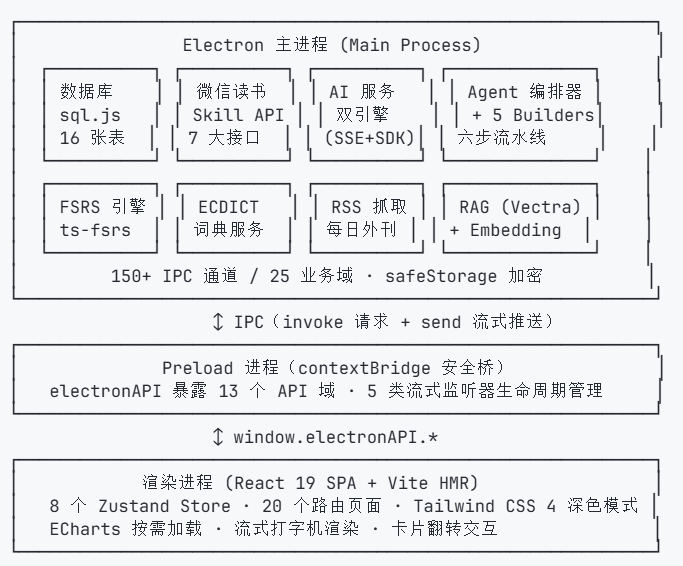
\includegraphics[width=0.32\textwidth]{figures/img_001.png}\hfill
    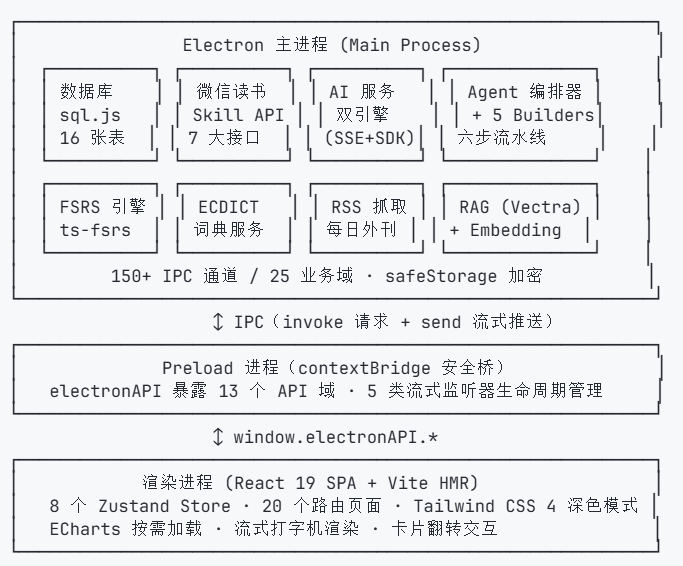
\includegraphics[width=0.32\textwidth]{figures/img_001.png}\hfill
    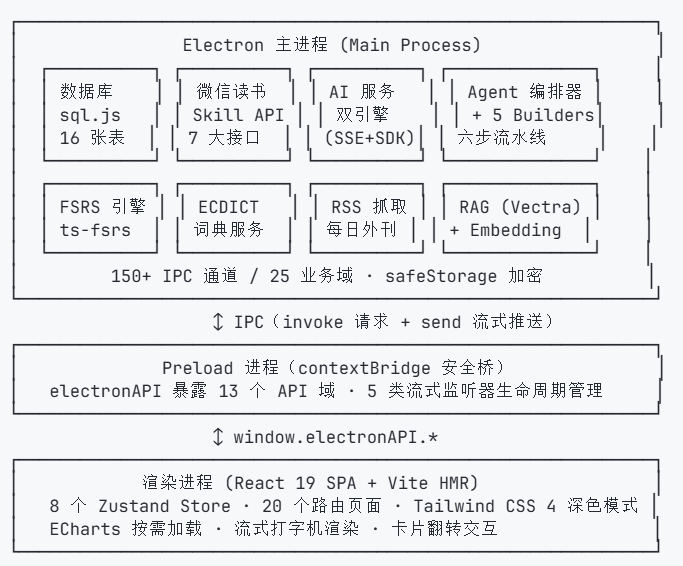
\includegraphics[width=0.32\textwidth]{figures/img_001.png}
    \caption{核心功能界面预览（示例：替换为 3 张主界面截图）}
    \label{fig:modules-preview}
\end{figure}

% --- 示意图/流程图专用占位（新增） ---
\begin{figure}[htbp]
    \centering
    
\includegraphics[width=0.95\textwidth]{figures/img_100.png}
    \caption{作品演示图 / 场景示意图（替换为你的作品演示图）}
    \label{fig:demo-scene}
\end{figure}

\begin{figure}[htbp]
    \centering
    
\includegraphics[width=0.95\textwidth]{figures/img_101.png}
    \caption{商业模式图 / 画布图（替换为你的商业模式图）}
    \label{fig:business-model}
\end{figure}

% --- 后续 5 大创新点 / 技术架构 / 重点专章的占位骨架（每节给出"风格提示 + 占位表格"） ---

\section{N 大核心创新点}
% 风格提示：每个创新点一节（subsection），先一段引出，再用 3-5 个加粗短句列举工程细节
\subsection{创新点 1：方法论自动注入 Agent（行业首创）}
{引文占位}传统 AI 阅读工具只能基于用户输入的上下文生成回答，无法主动调用书中的结构化方法论。本作品引入 \texttt{MethodologyContextBuilder}：

\begin{itemize}
    \item 从书籍对应的 methodology 表检索相关方法论
    \item 按意图相关性排序后注入 system prompt
    \item AI 回答时自动引用具体章节与方法论名称
    \item 对话结束后回调更新掌握度（mastery level）
\end{itemize}

\subhead{效果}回答不再泛泛而谈，而是基于书籍知识框架给出可操作建议，并持续追踪用户对每条方法论的掌握程度。

\subsection{创新点 2：5 维 ContextBuilder（预算制懒加载）}
{引文占位}为降低 Token 消耗并提升回答相关性，构建 5 个上下文维度，按优先级懒加载。

\begin{table}[htbp]
\centering
\begin{tabularx}{\textwidth}{c >{\bfseries}l X c}
\toprule
\textbf{优先级} & \textbf{构建器} & \textbf{数据源} & \textbf{Token 预算} \\
\midrule
90 & BookContextBuilder & 语义搜索 + 关键词回退 & 1500 \\
80 & MethodologyContextBuilder & 相关性评分 Top 5 & 1000 \\
70 & KnowledgeCardContextBuilder & 相关性评分 Top 10 & 800 \\
50 & MemoryContextBuilder & 相关记忆 3 条 + 摘要 & 500 \\
40 & UserProfileContextBuilder & 动态生成画像 & 200 \\
\bottomrule
\end{tabularx}
\caption{5 维 ContextBuilder 配置（预算共 4000 tokens）}
\label{tab:context-builder}
\end{table}

\subhead{三条硬规则}预算不足时低优先级自动跳过；每个构建器独立失败不拖垮整体（fail-soft 柔性容错）；超预算截断并显式标记。

\subsection{创新点 3：FSRS v5 间隔复习}
{占位}简要说明：算法出处、与 Anki 同源、DSR 模型、自动喂卡、零破坏升级。

\subsection{创新点 4：本地优先架构}
{占位}简要说明：全本地 SQLite、Electron safeStorage 加密、AI 热切换、零遥测。

\subsection{创新点 5：ECDICT 离线词典 + 语境化英语学习}
{占位}简要说明：13.6MB JSON、悬停查词、6 类词形变化、RSS 外刊、加入生词本后由 FSRS 调度。

\section{整体技术架构}

\subsection{系统架构总览}
% 风格提示：放 1 张大图（3840x3000 类），下方 1 段注解
\begin{figure}[htbp]
    \centering
    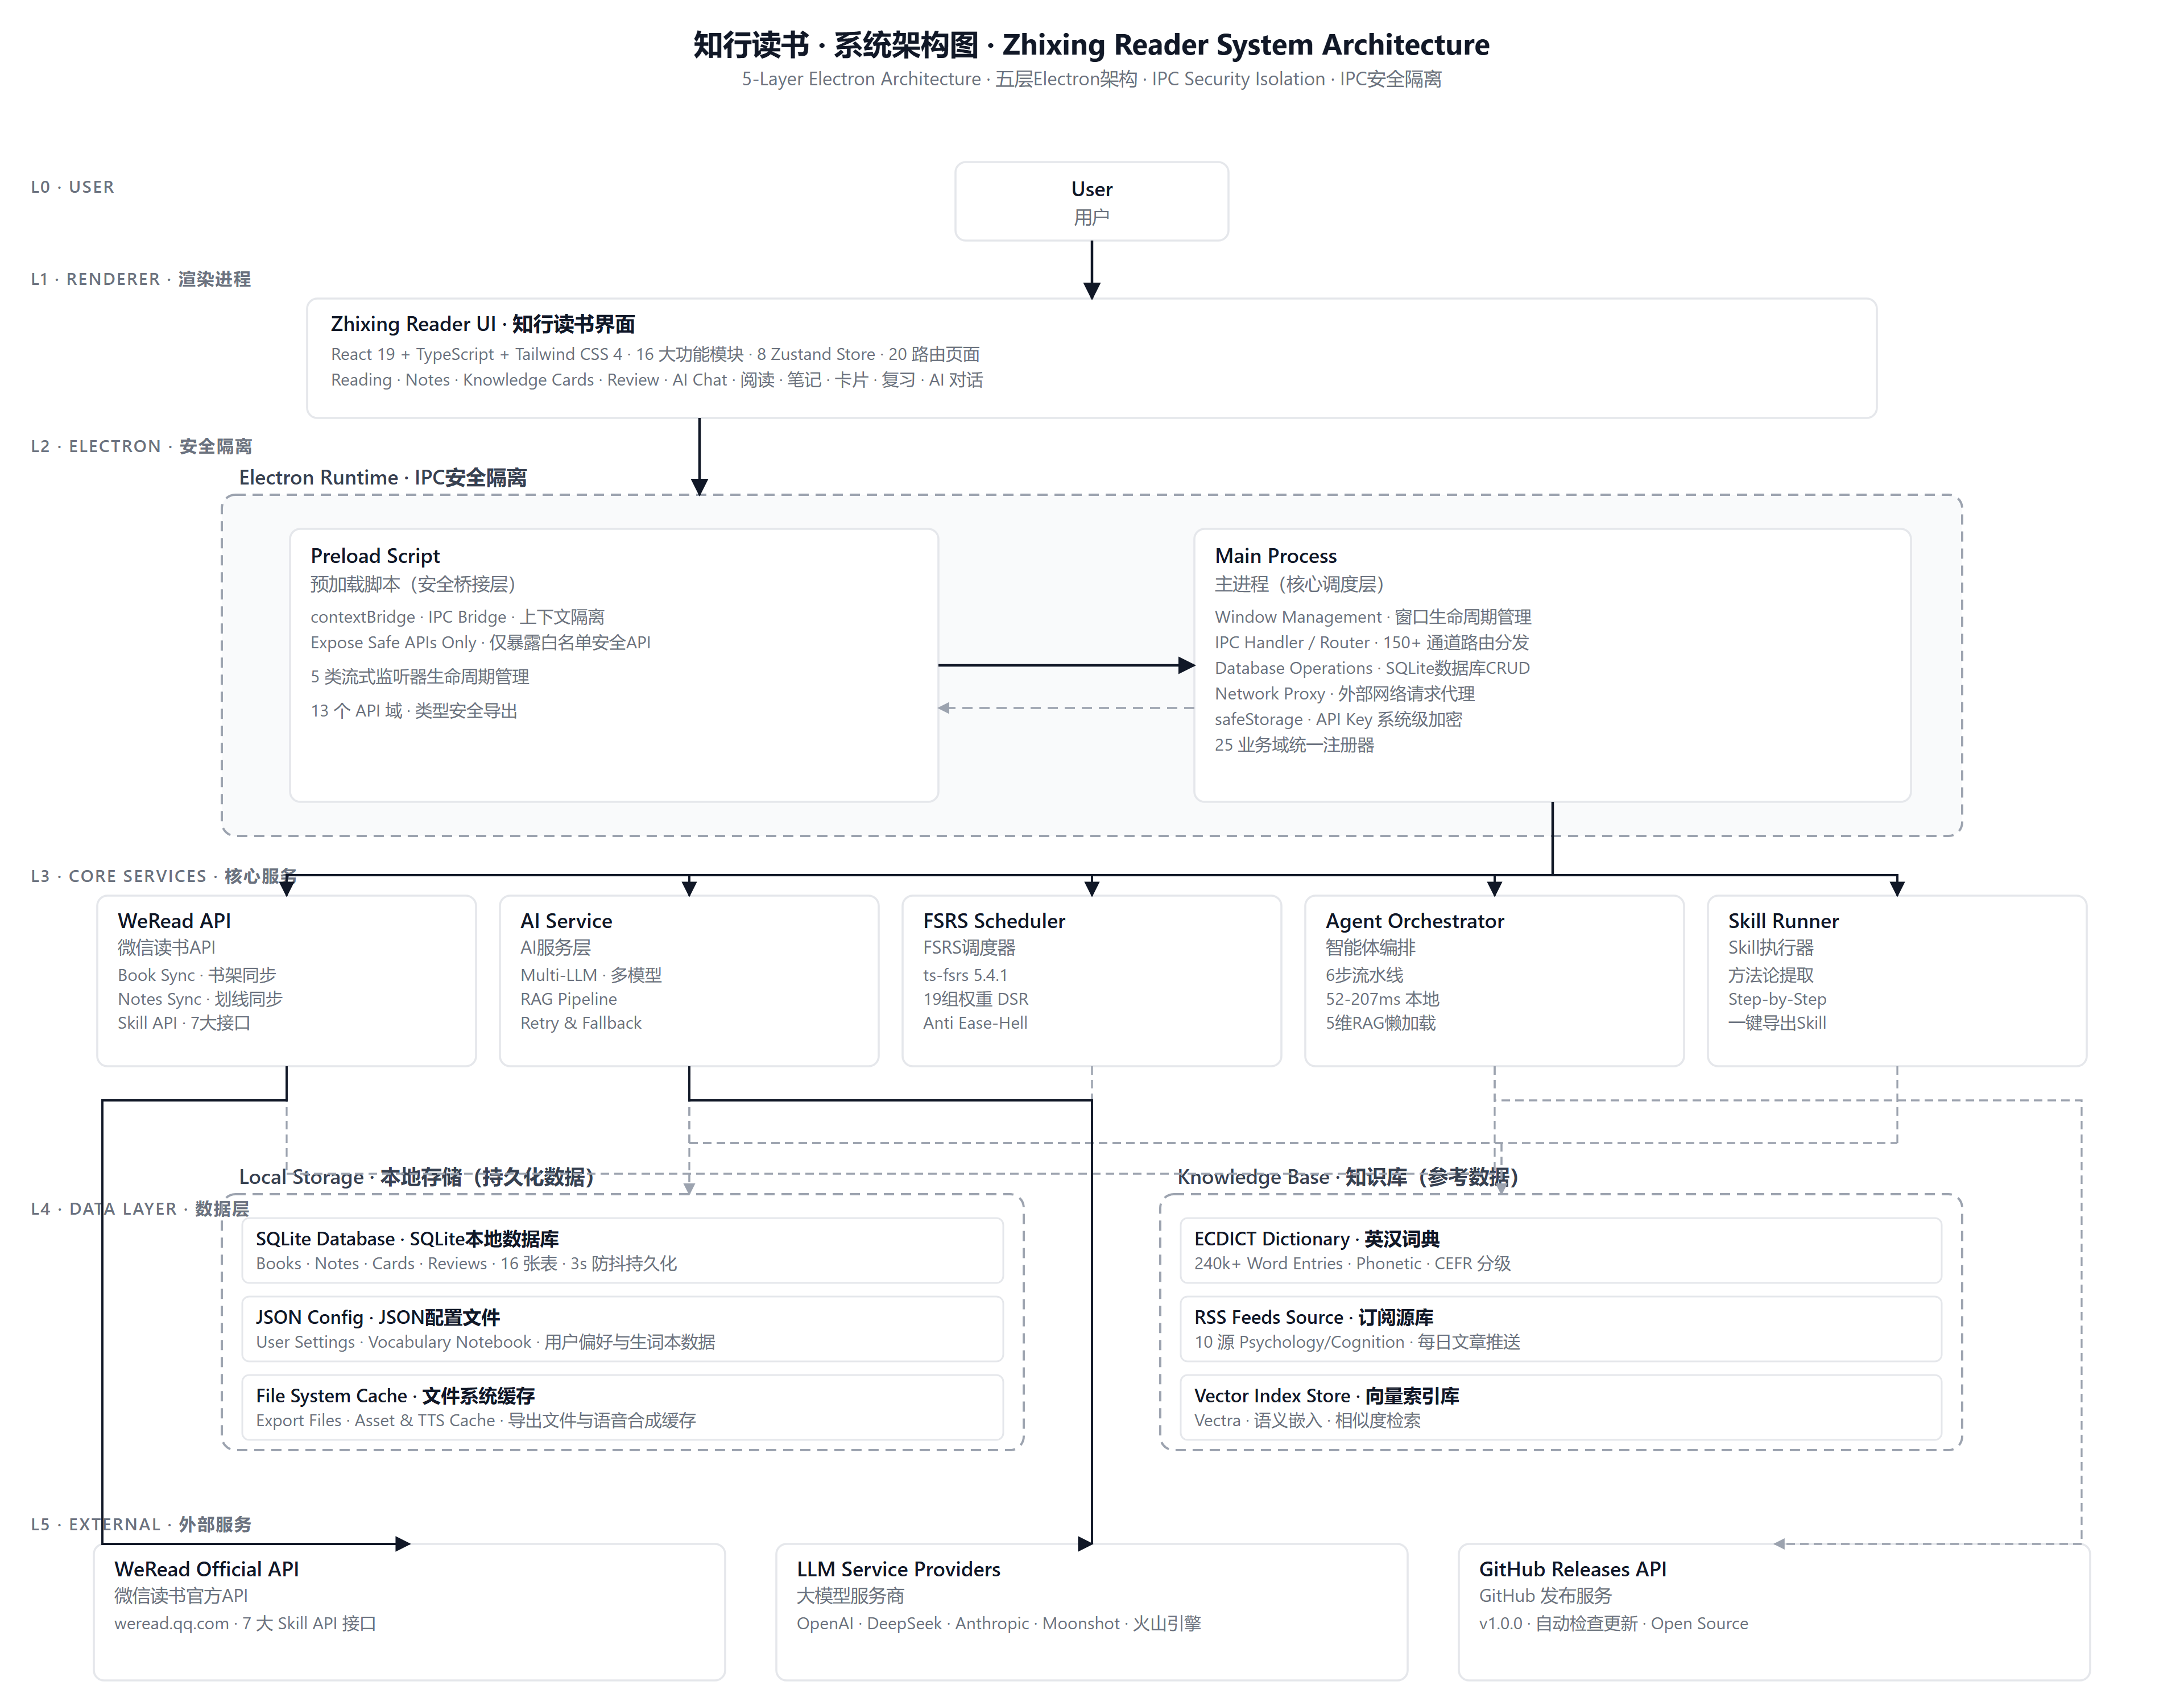
\includegraphics[width=0.95\textwidth]{figures/img_000.png}
    \caption{系统架构总览图}
    \label{fig:arch-overview}
\end{figure}

\subsection{三进程架构}
% 风格提示：放 1 张相对小的图（683x566 类），下方注释放性能/安全注解
\begin{figure}[htbp]
    \centering
    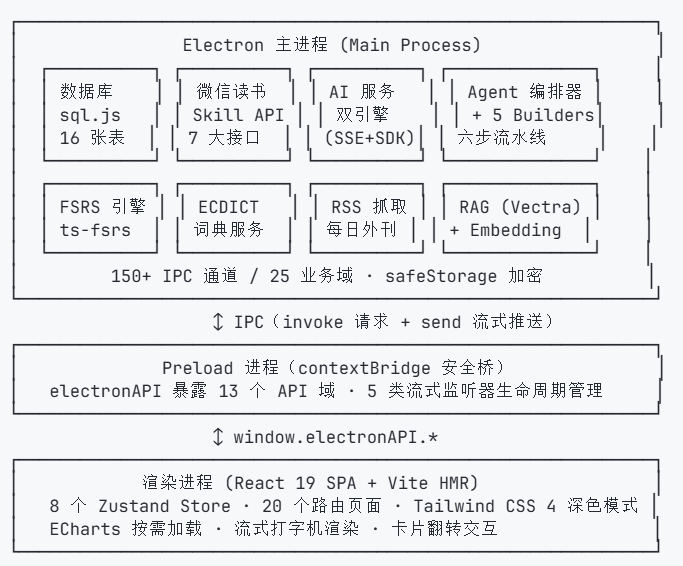
\includegraphics[width=0.55\textwidth]{figures/img_001.png}
    \caption{三进程架构总览}
    \label{fig:three-process}
\end{figure}

\subhead{多模型深度思考归一化}一套代码兼容三家模型的"深度思考"输出格式（DeepSeek R1 的 \texttt{reasoning\_content}、OpenAI o 系列的 \texttt{reasoning.summary}、Claude 的 \texttt{thinking\_delta}）。归一化层统一转换后，一套折叠面板 UI 通吃，并支持随时中断生成（立即中止 + 柔性停止双模式）。

\subsection{IPC 通信架构}
\begin{figure}[htbp]
    \centering
    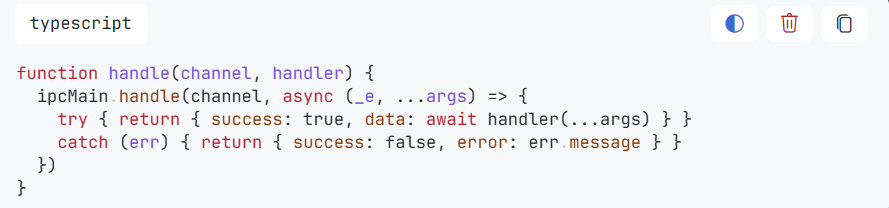
\includegraphics[width=0.85\textwidth]{figures/img_002.png}
    \caption{IPC 通信架构（N 通道 / N 业务域）}
    \label{fig:ipc}
\end{figure}

{占位}所有通道走统一注册器，天然获得一致的错误处理与类型安全。流式场景采用反向推送 4 类事件（CHUNK / REASONING\_CHUNK / COMPLETE / ERROR），杜绝监听器泄漏。

\subsection{数据库设计}
\begin{table}[htbp]
\centering
\begin{tabularx}{\textwidth}{>{\bfseries}l X X}
\toprule
\textbf{关键表} & \textbf{用途} & \textbf{设计亮点} \\
\midrule
books / highlights & 书籍与划线 & 与上游增量合并、内容指纹去重 \\
cards / reviews & FSRS 卡片与复习日志 & schema 与 Anki 对齐 \\
knowledge\_cards / methodologies & 知识卡片与方法论 & AI 蒸馏 + 掌握度追踪 \\
memories & AI 长期记忆 & 偏好/事实/反馈三类，按重要度检索 \\
conversations / chat\_messages & 对话 & 点赞/收藏/意图/Bloom 层级全记录 \\
token\_usage / daily\_stats & 用量与学习统计 & 成本核算到每次请求 \\
\bottomrule
\end{tabularx}
\caption{数据库核心表（16 张）}
\label{tab:database}
\end{table}

\subsection{技术栈层次}
\begin{table}[htbp]
\centering
\begin{tabularx}{\textwidth}{>{\bfseries}l X X}
\toprule
\textbf{层} & \textbf{选型} & \textbf{说明} \\
\midrule
桌面壳 & Electron 35 + electron-vite 2 & 三进程隔离，Vite HMR \\
UI & React 19 + React Router 7 + Tailwind CSS 4 & 路由懒加载，启动 < 1 秒 \\
状态 & Zustand 5 & 乐观更新 + 流式控制 \\
类型 & TypeScript 5.6 strict & 50,000+ 行全量严格模式 \\
数据 & sql.js（SQLite WASM）+ Vectra 向量索引 & 双引擎全本地 \\
记忆算法 & ts-fsrs 5.4.1 & Anki 同源 FSRS v5 \\
AI & Vercel AI SDK + 自研 SSE 引擎 & 多服务商热切换 + reasoning 归一化 \\
图表 & Apache ECharts（按需引入） & 第三方库独立打包 \\
质量 & Vitest 2 + coverage-v8 & N 个用例 / N\% 覆盖率 \\
打包 & electron-builder + NSIS & 已发布 v1.0.0 \\
\bottomrule
\end{tabularx}
\caption{技术栈层次详情}
\label{tab:tech-stack}
\end{table}

\section{重点专章：核心引擎/算法/机制}
% 风格提示：这是"灵魂模块"，要单独突出，1 张大流程图 + 1 张时序图 + 每步细节
\subsection{全景流程}
\begin{figure}[htbp]
    \centering
    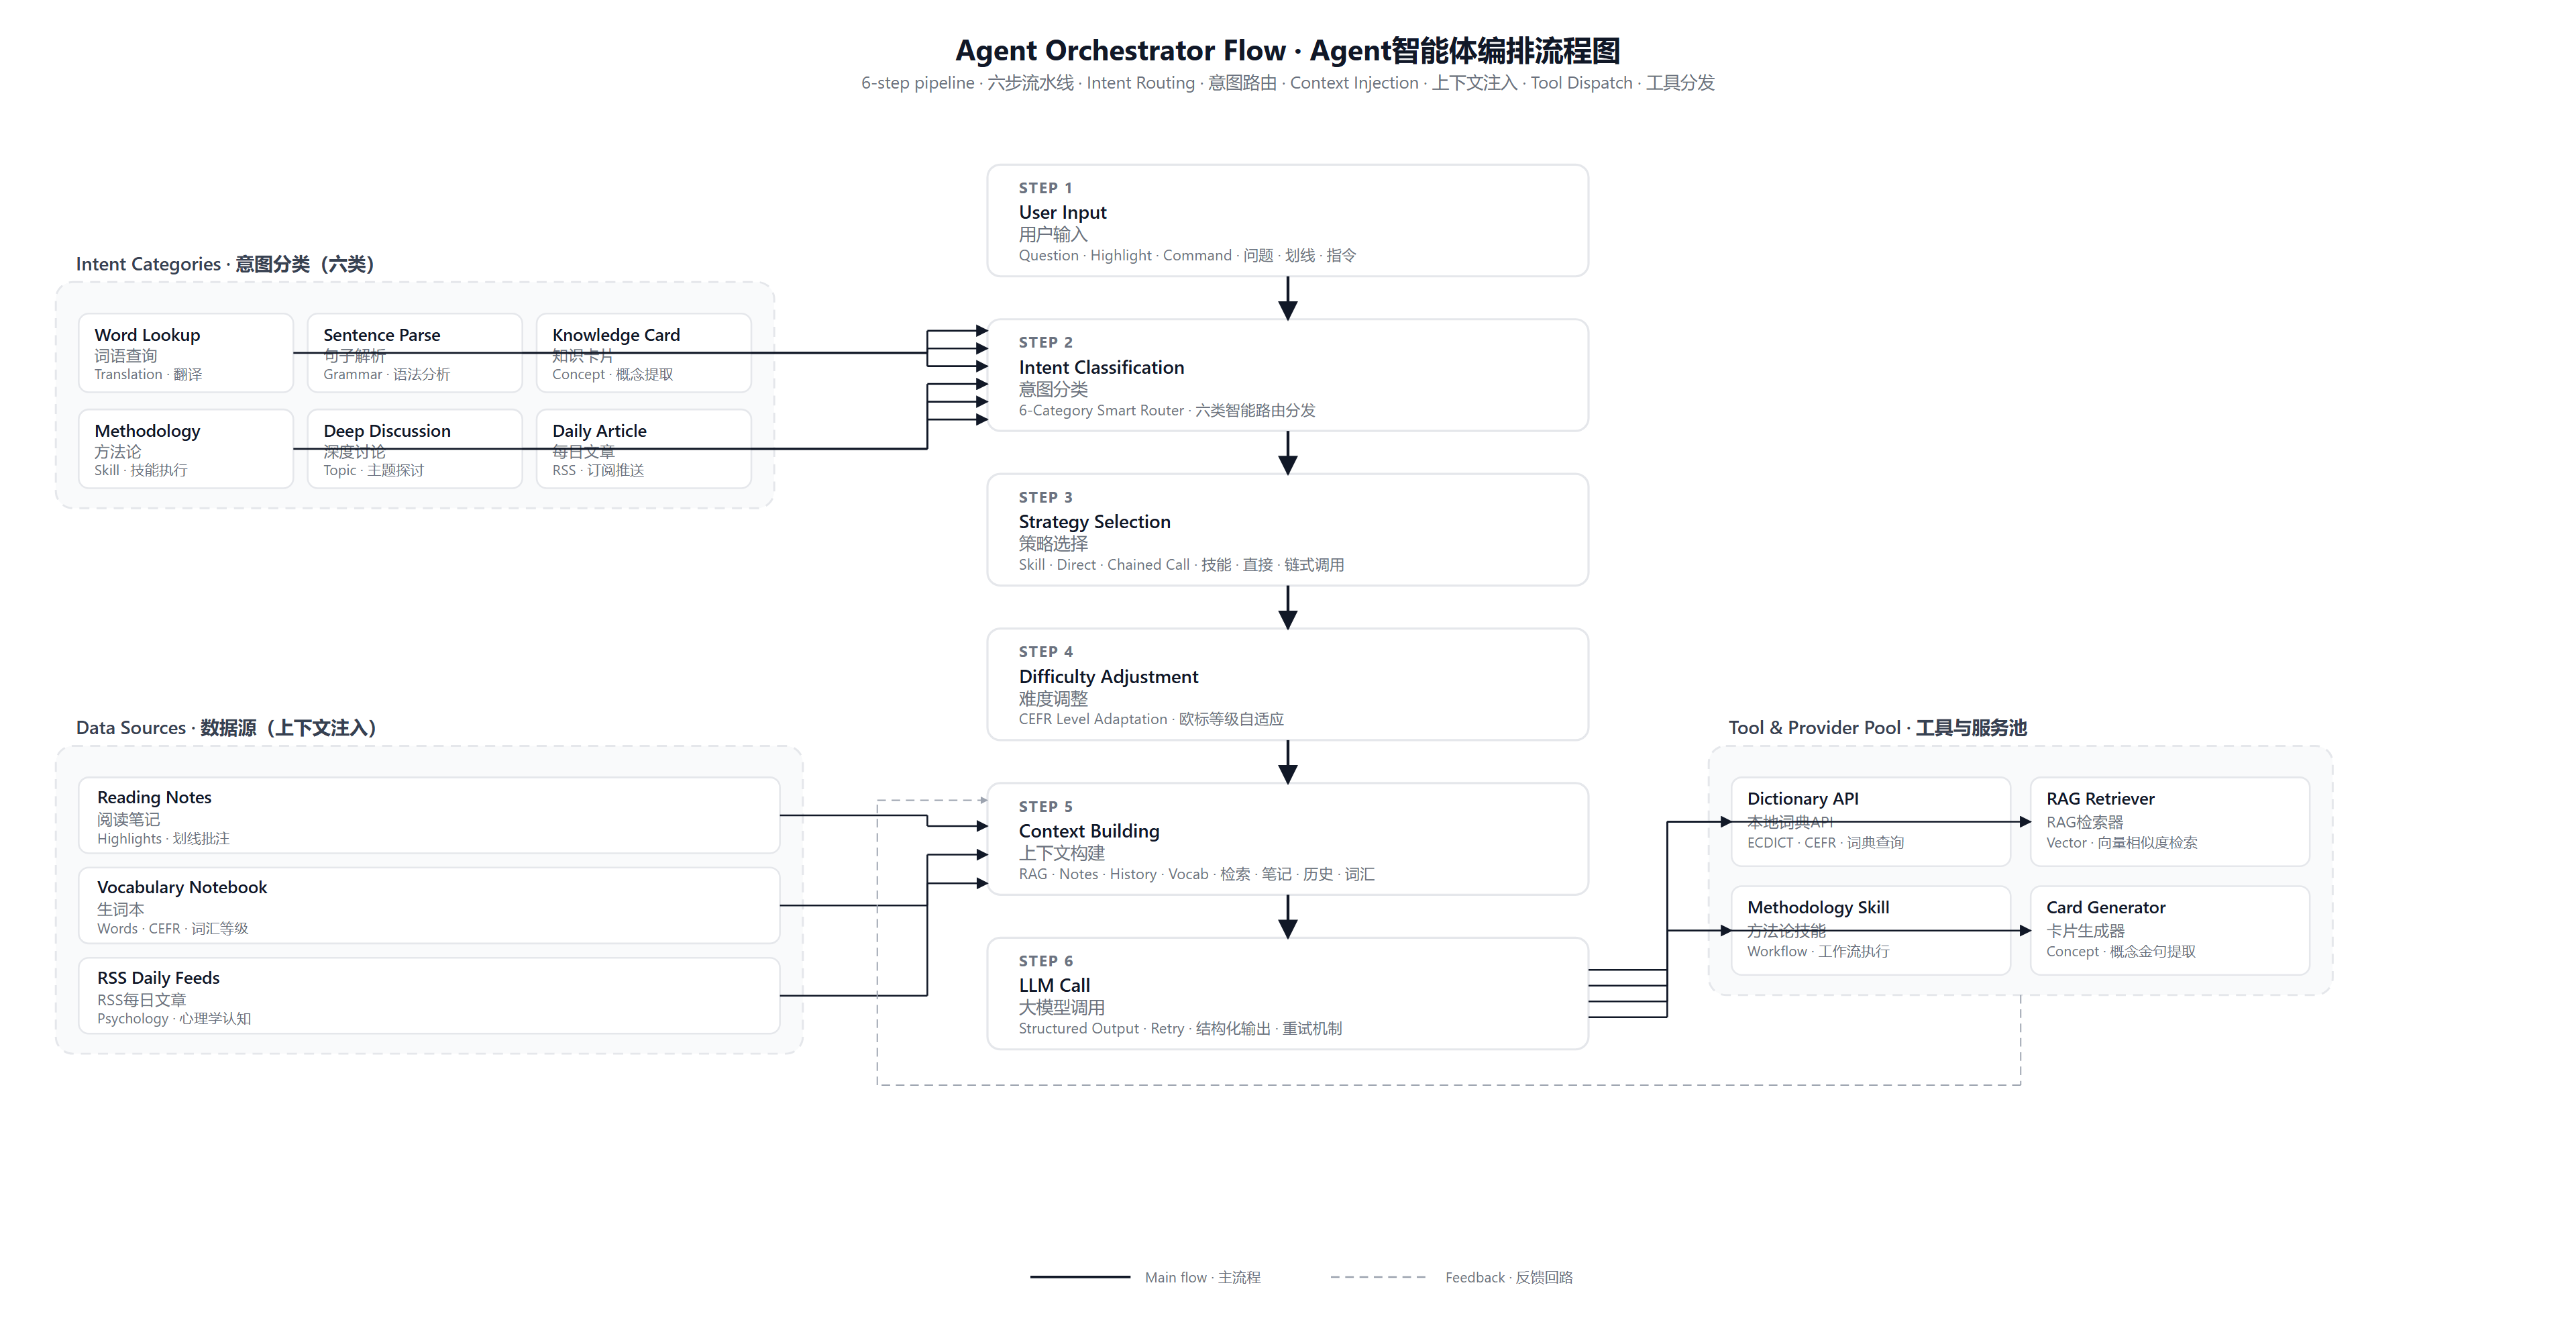
\includegraphics[width=0.95\textwidth]{figures/img_003.png}
    \caption{核心引擎/算法流程图（替换为你的流程图）}
    \label{fig:core-flow}
\end{figure}

\begin{figure}[htbp]
    \centering
    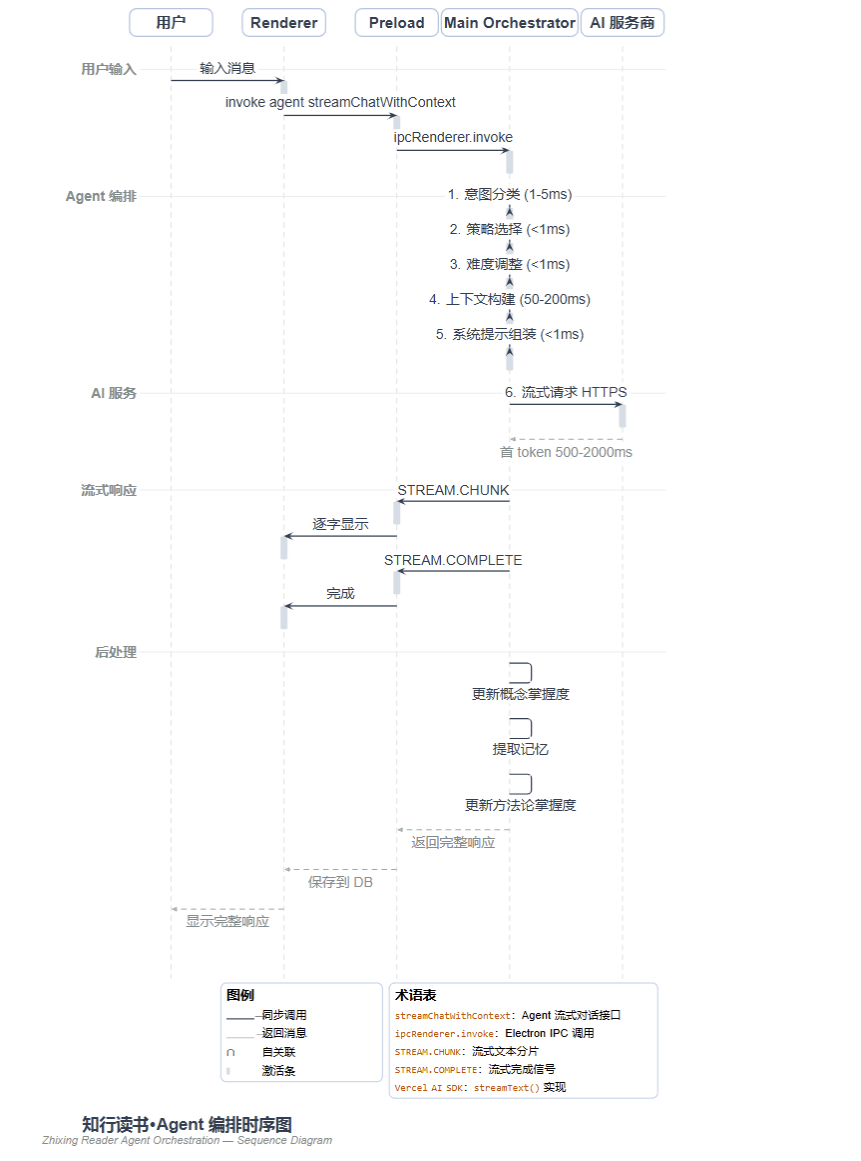
\includegraphics[width=0.45\textwidth]{figures/img_004.png}
    \caption{核心引擎/算法时序图（替换为你的时序图）}
    \label{fig:core-sequence}
\end{figure}

\subsection{每一步的设计细节}
\subhead{步骤 1：xxx}{占位}说明输入、处理逻辑、输出。
\subhead{步骤 2：xxx}{占位}说明输入、处理逻辑、输出。
\subhead{步骤 3：xxx}{占位}说明输入、处理逻辑、输出。

\subsection{性能画像}
\begin{table}[htbp]
\centering
\begin{tabularx}{\textwidth}{>{\bfseries}l X X}
\toprule
\textbf{步骤} & \textbf{延迟} & \textbf{类型} \\
\midrule
步骤 1 & N\,ms & 本地计算 / 网络请求 \\
步骤 2 & N\,ms & 本地计算 / 网络请求 \\
步骤 3 & N\,ms & 本地计算 / 网络请求 \\
合计 & N\,ms & 全链路 \\
\bottomrule
\end{tabularx}
\caption{核心引擎/算法性能画像}
\label{tab:perf}
\end{table}

% =====================================================================
% 第 3 章：附言（可选模块库）
% =====================================================================
\chapter{附言}

\ifshowtools
\section{工具使用与经验总结}
\subsection{使用截图与会话 ID 概览}
{引文占位}本项目历经多次迭代，使用 Trae IDE 和 Trae work 集中开发；期间报名了 Trae 创造力大赛，前端使用 Trae Design 进行设计重构。以下是部分使用截图和部分会话 ID 概览。

\subhead{Trae IDE}
\begin{figure}[htbp]
    \centering
    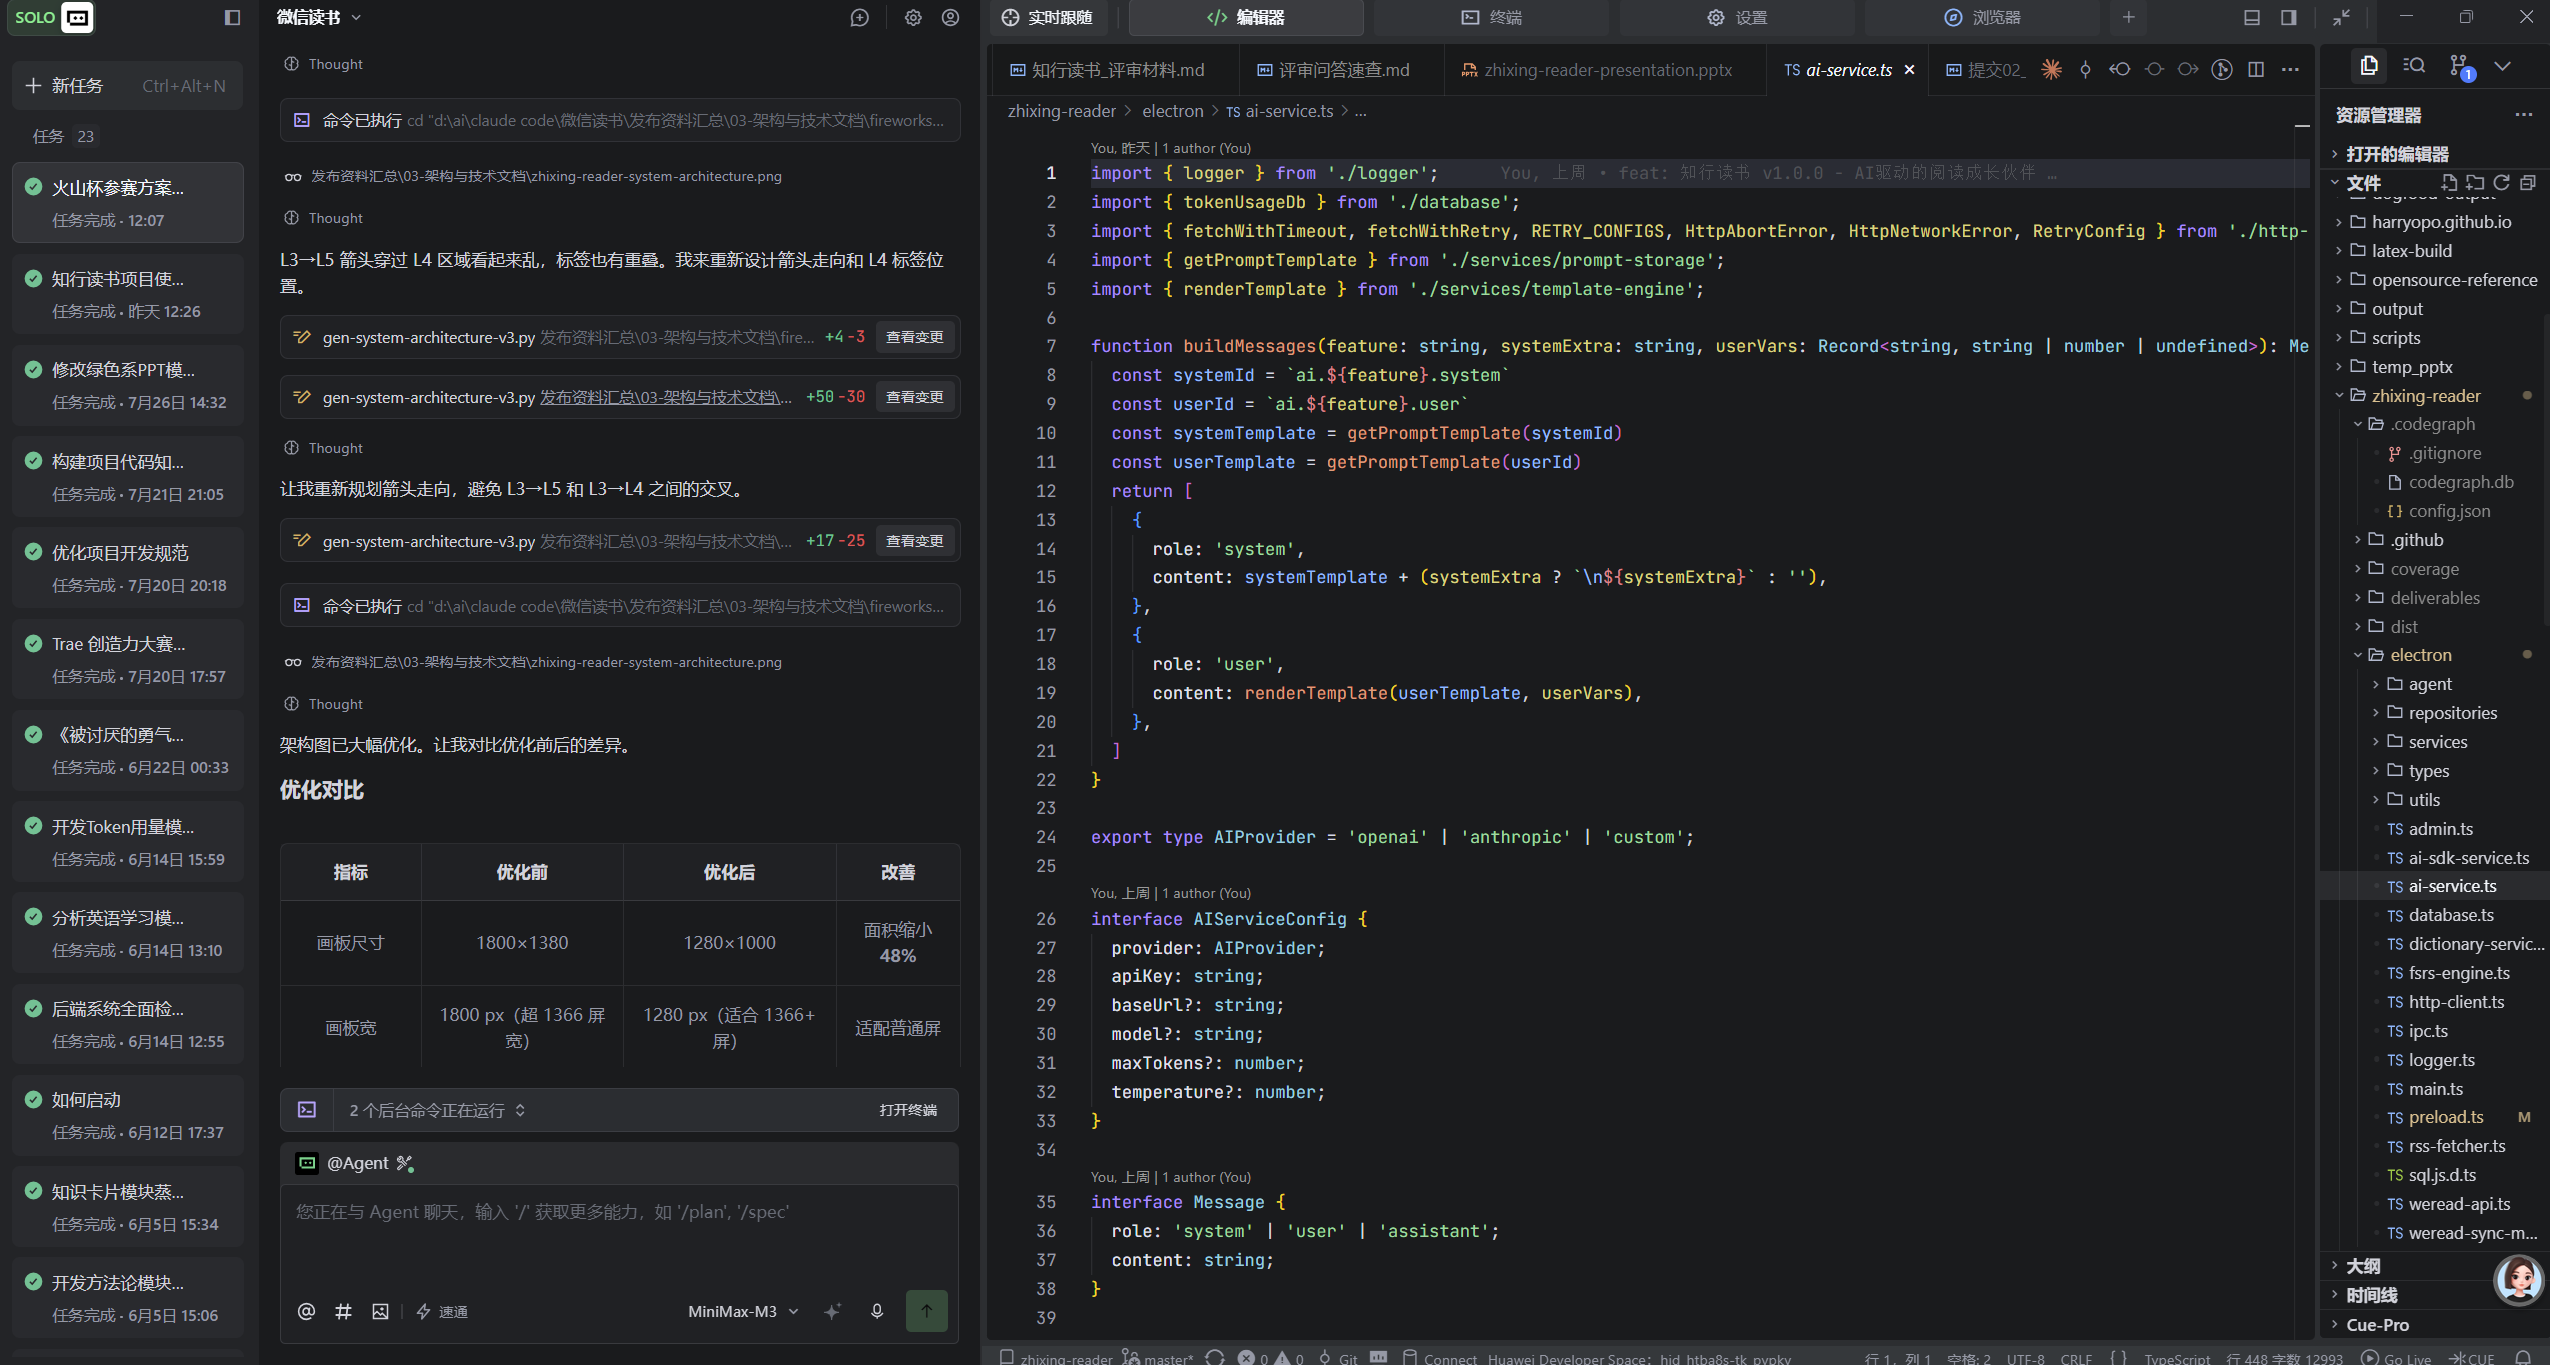
\includegraphics[width=0.48\textwidth]{figures/img_005.png}\hfill
    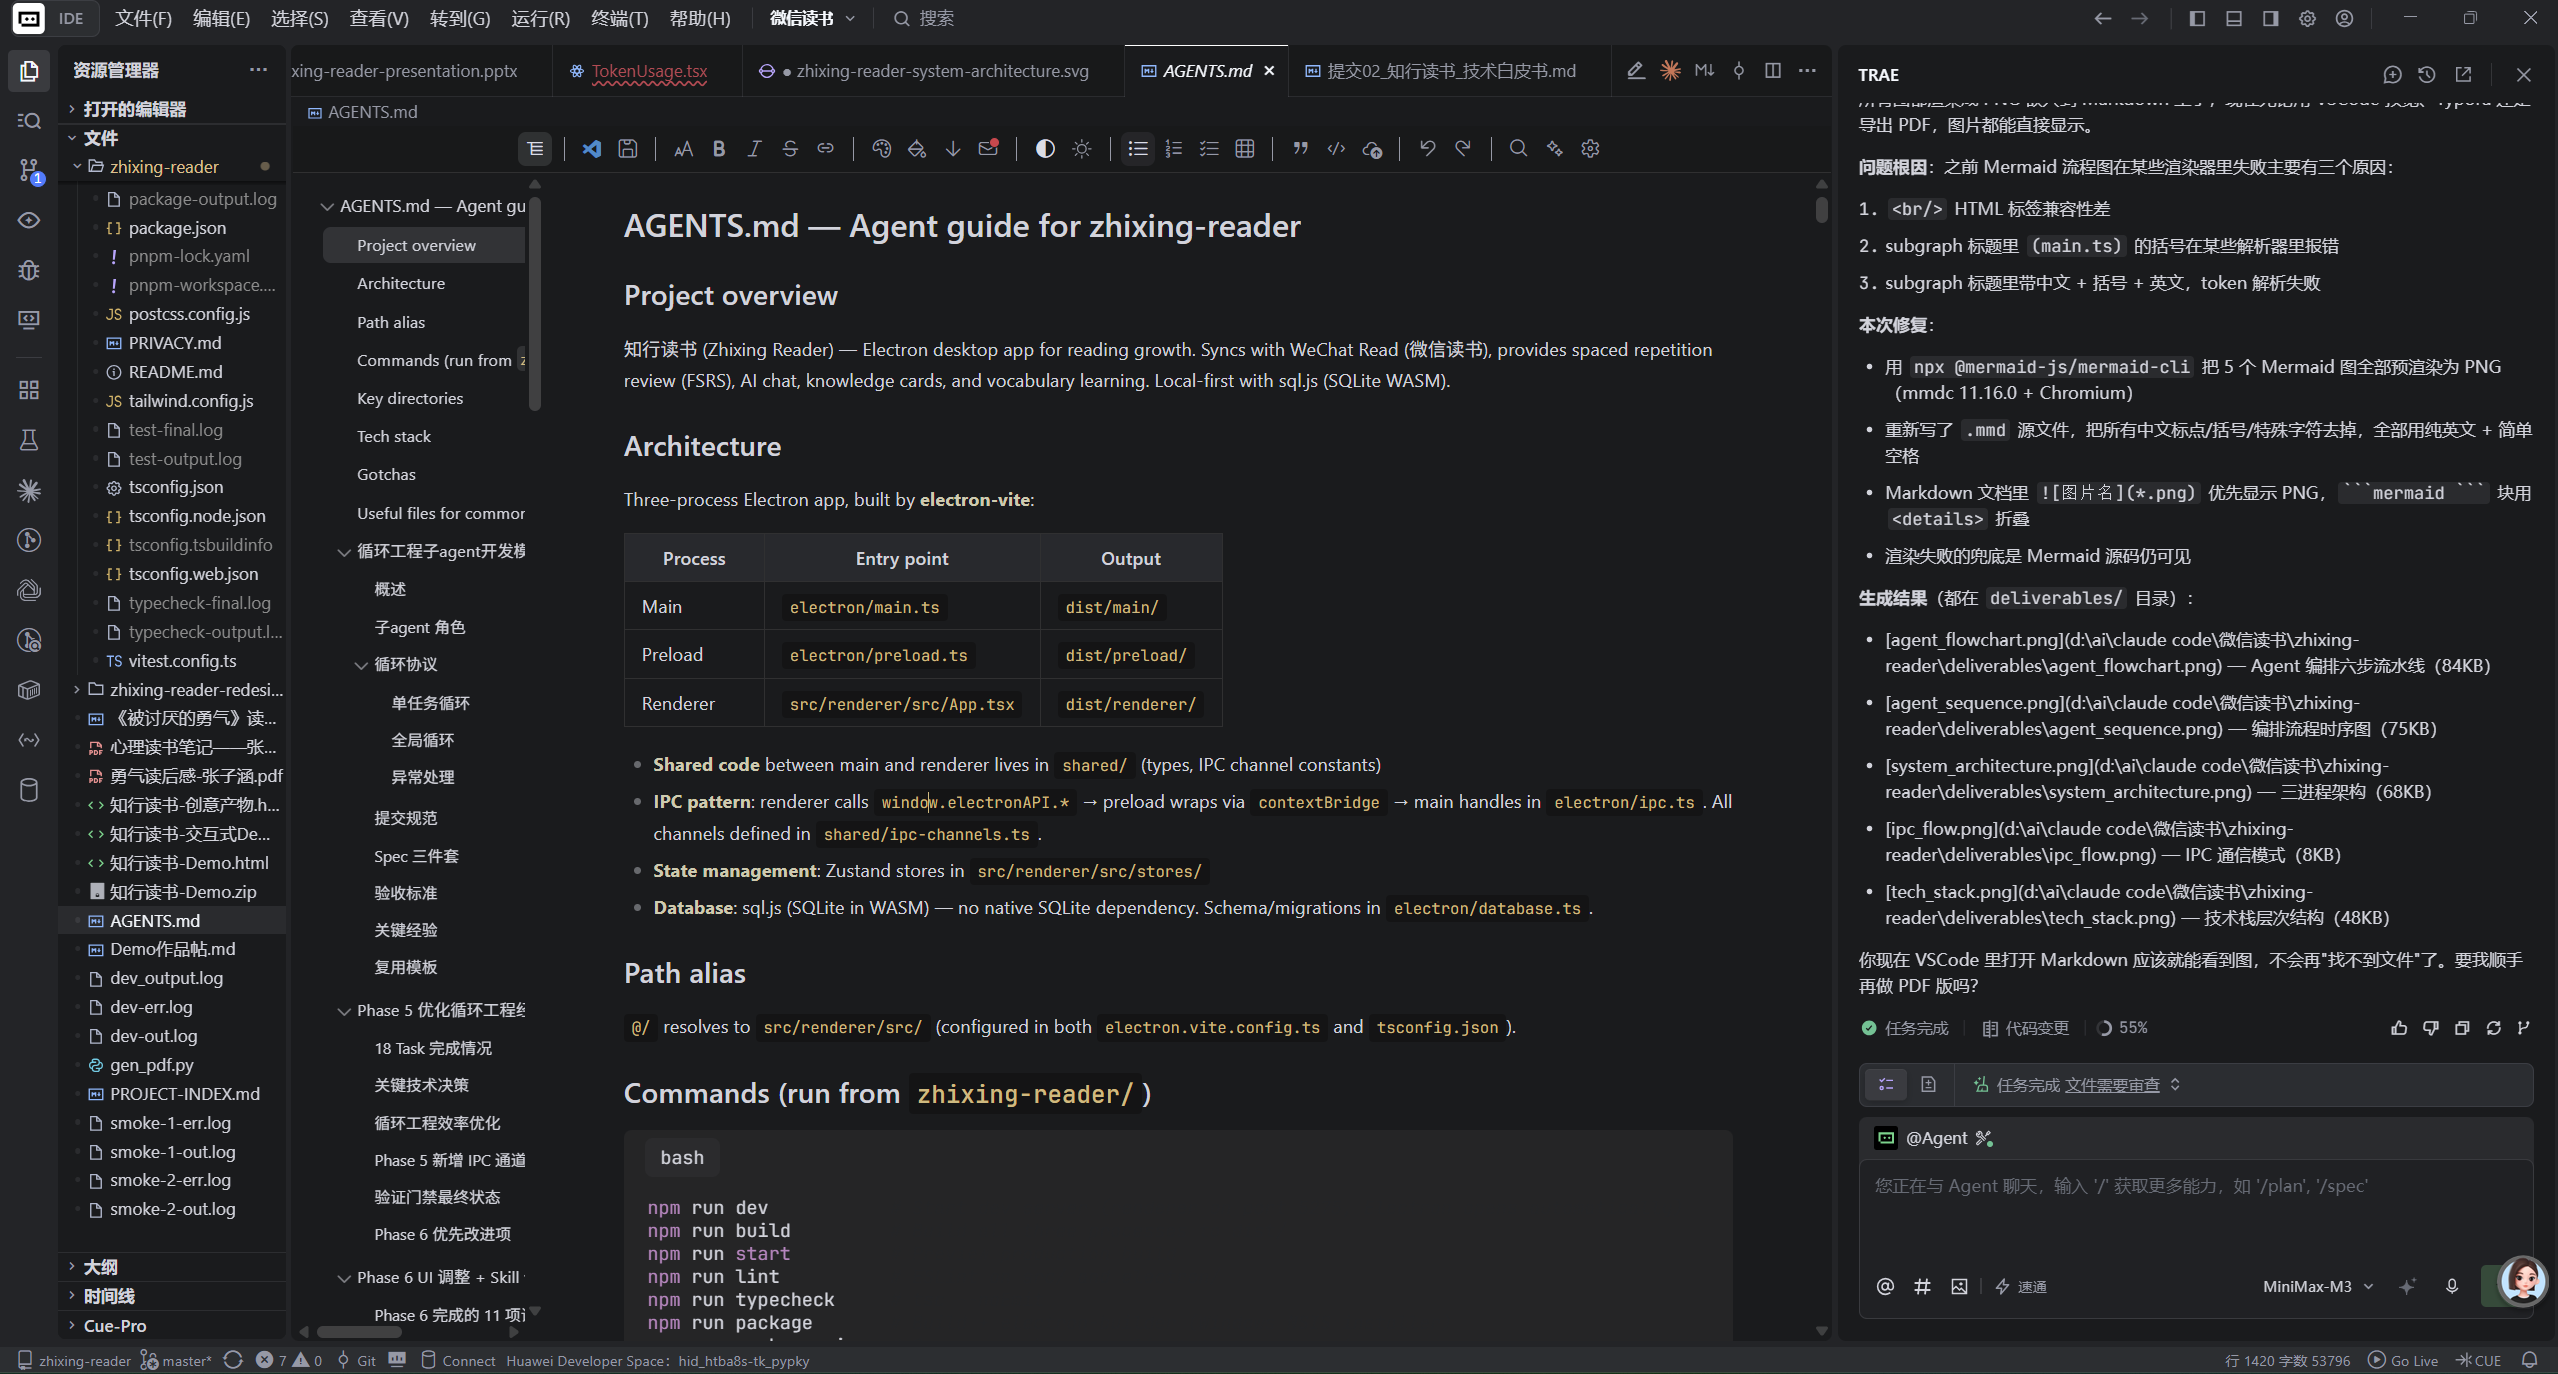
\includegraphics[width=0.48\textwidth]{figures/img_006.png}\\[6pt]
    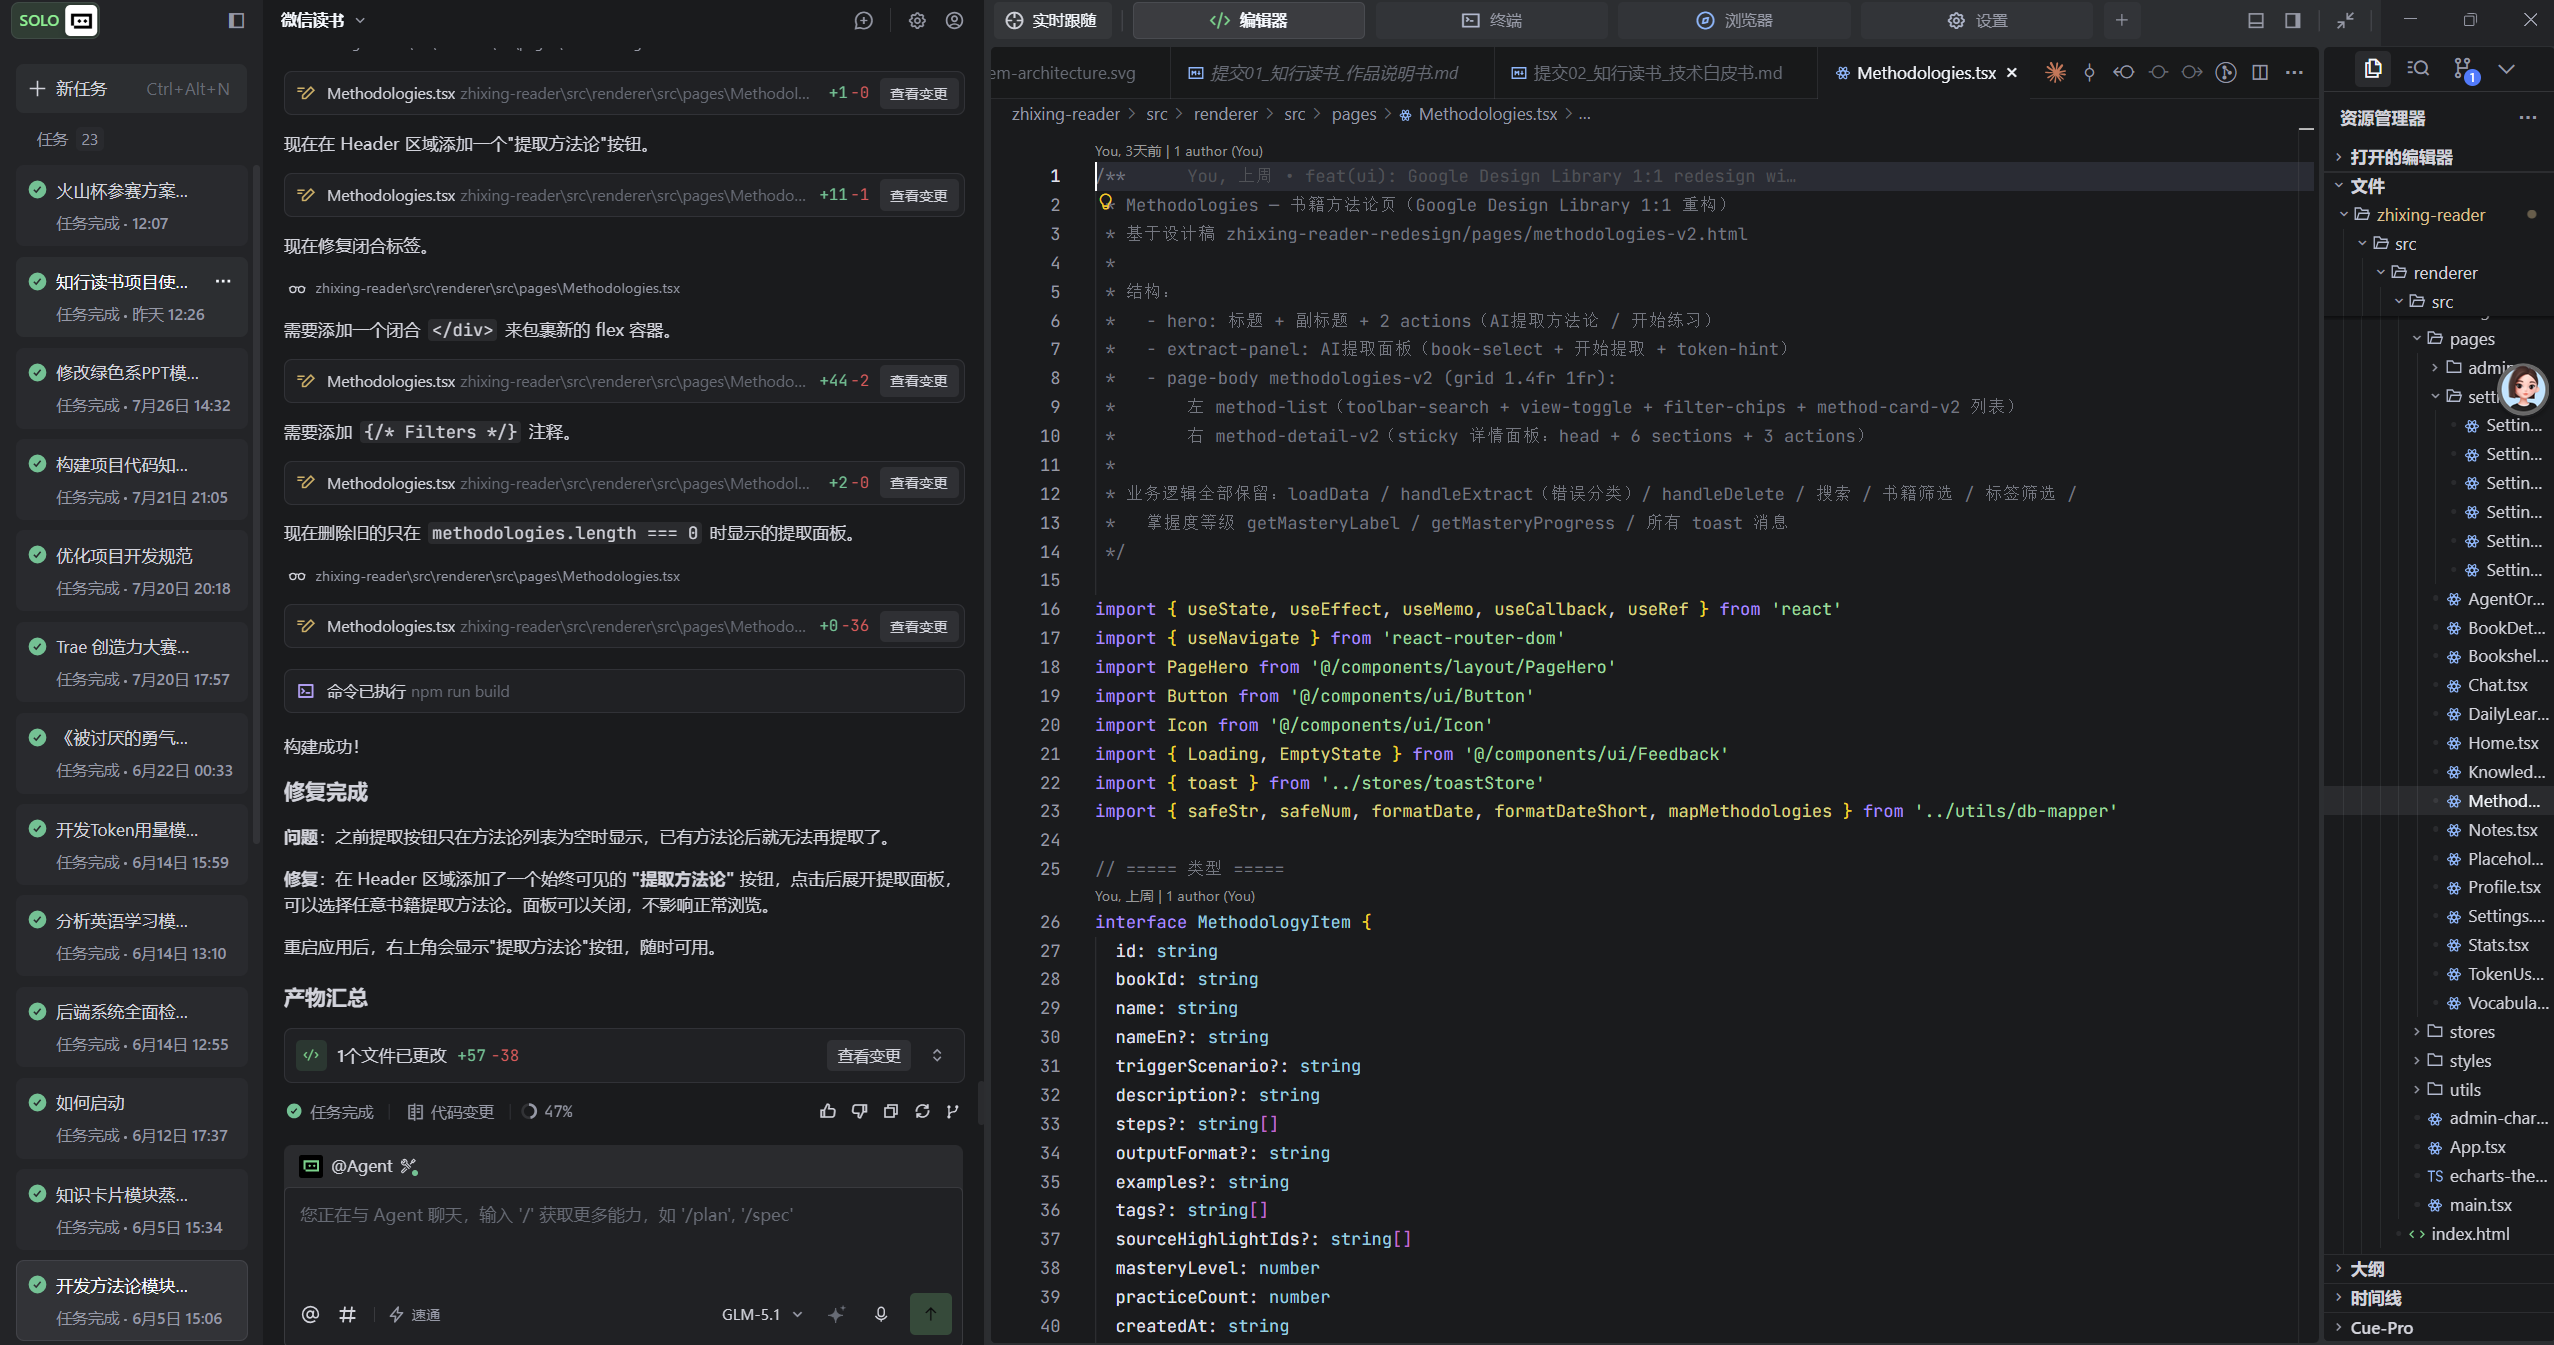
\includegraphics[width=0.48\textwidth]{figures/img_007.png}\hfill
    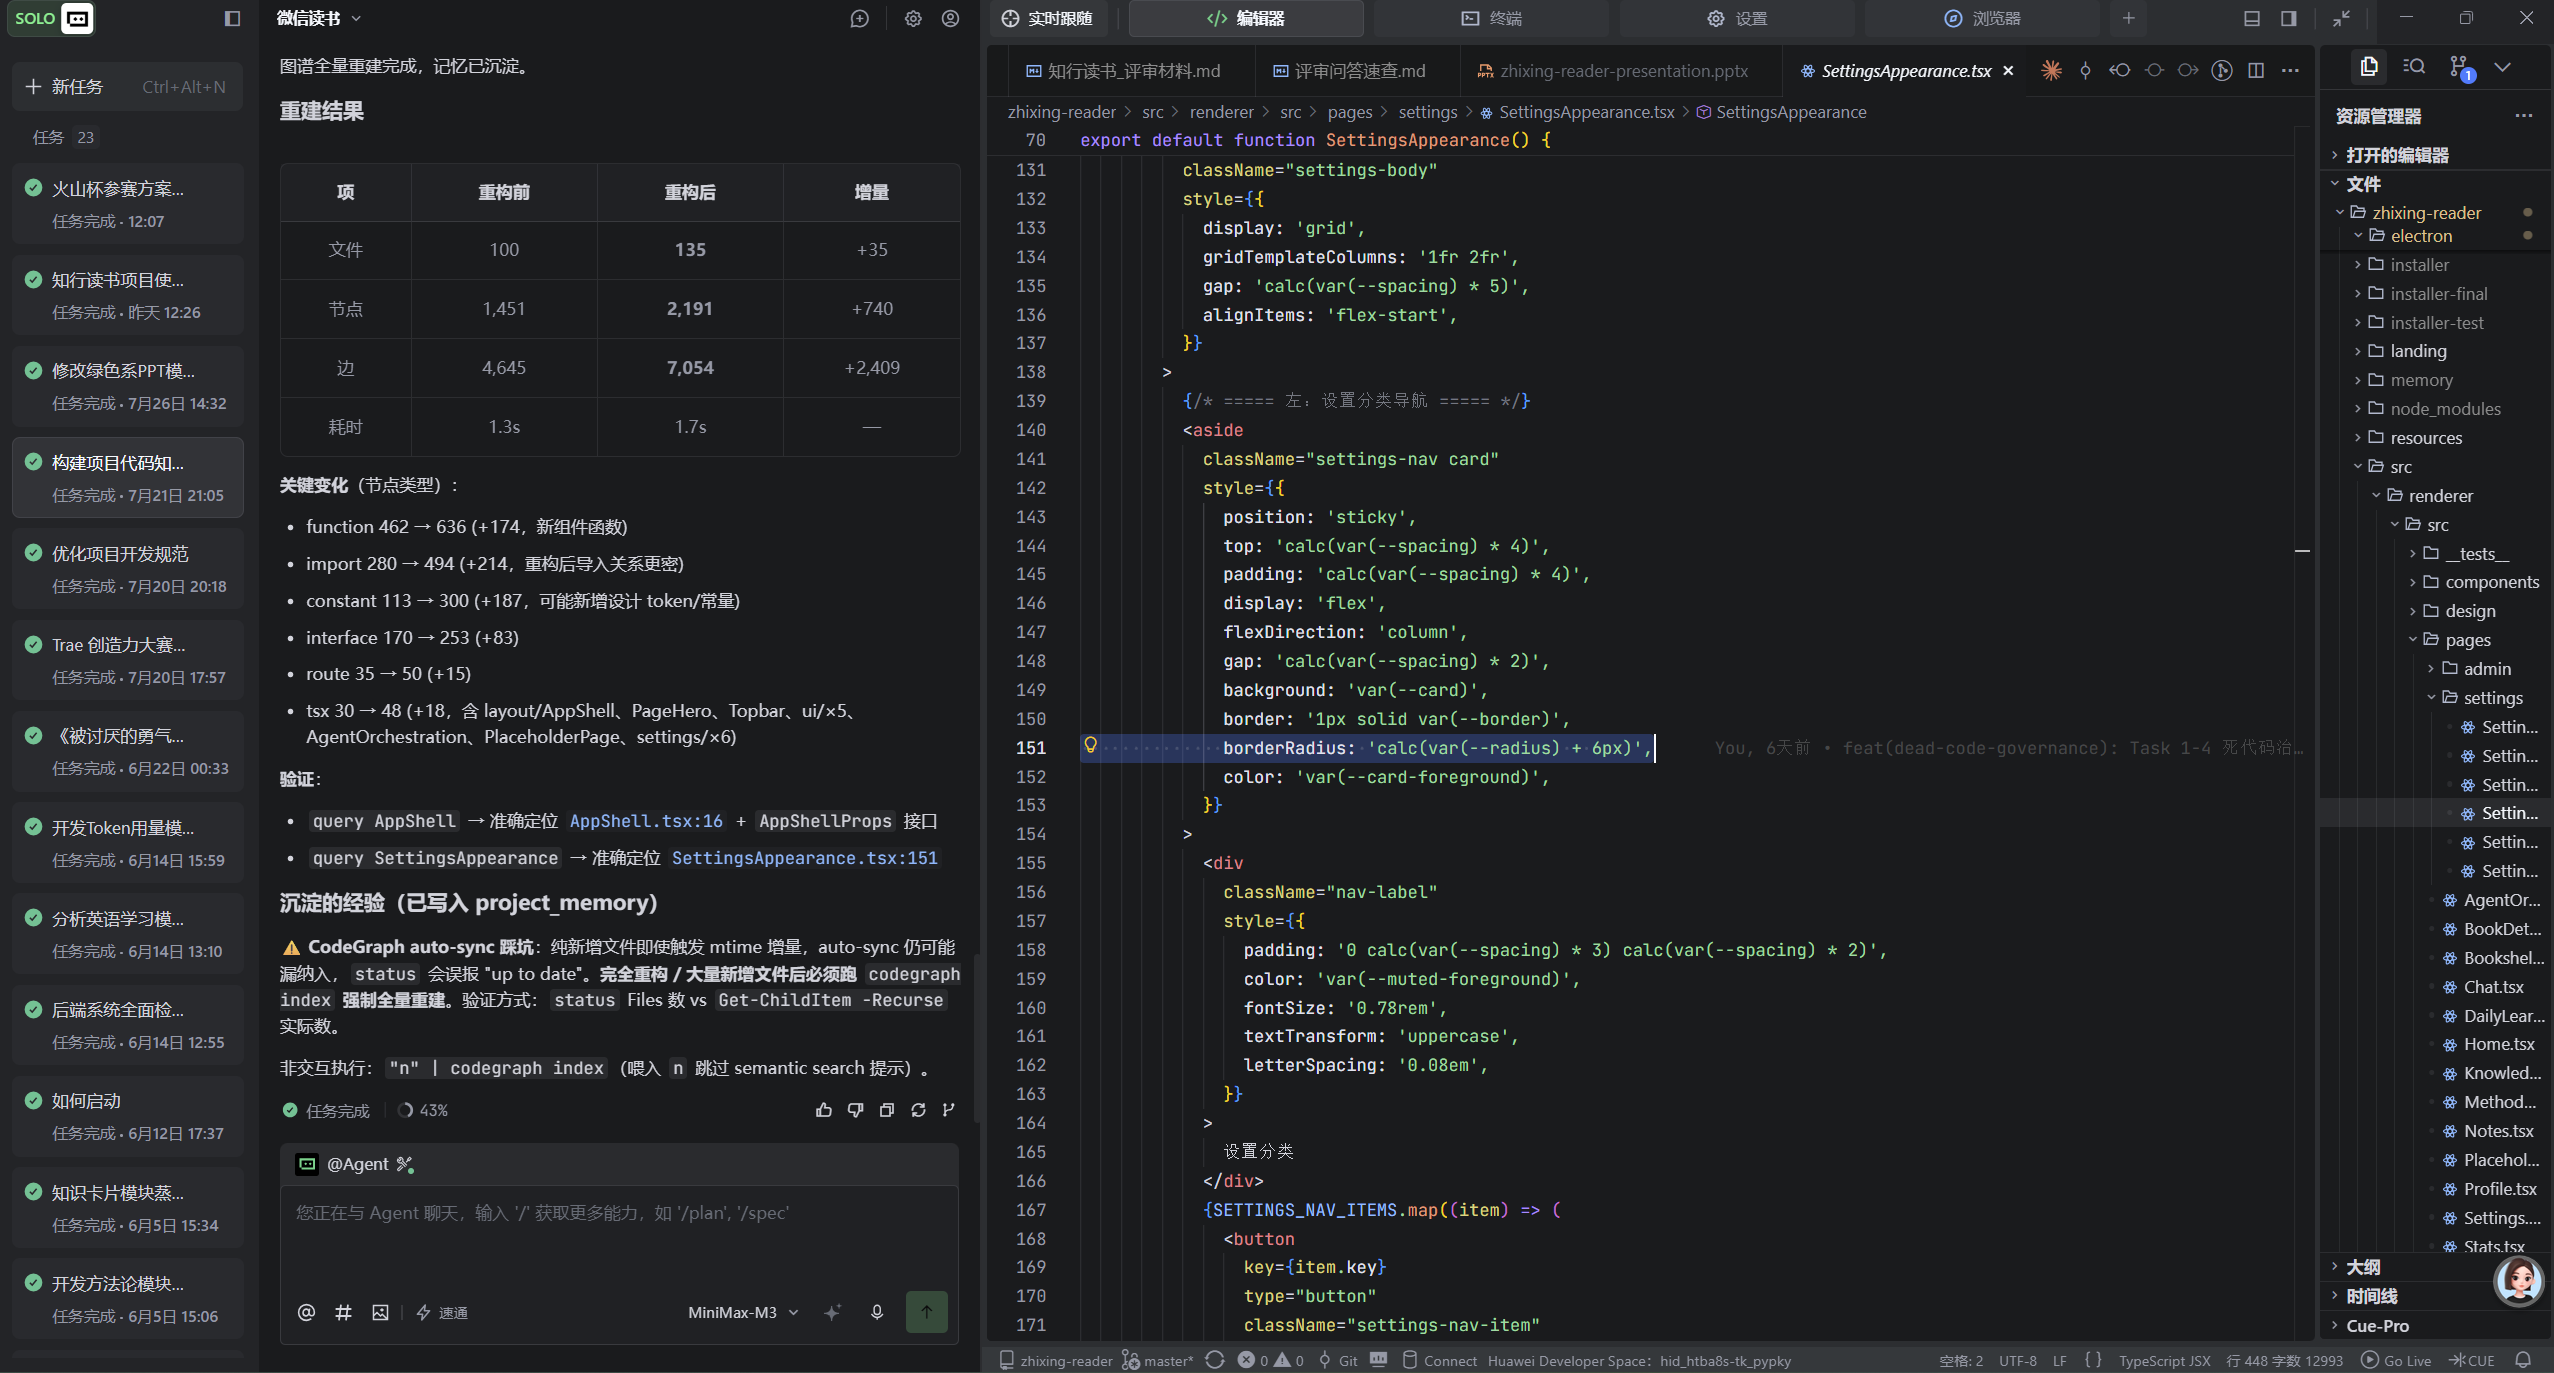
\includegraphics[width=0.48\textwidth]{figures/img_008.png}
    \caption{Trae IDE 使用截图（4 张）}
    \label{fig:trae-ide-1}
\end{figure}

\begin{figure}[htbp]
    \centering
    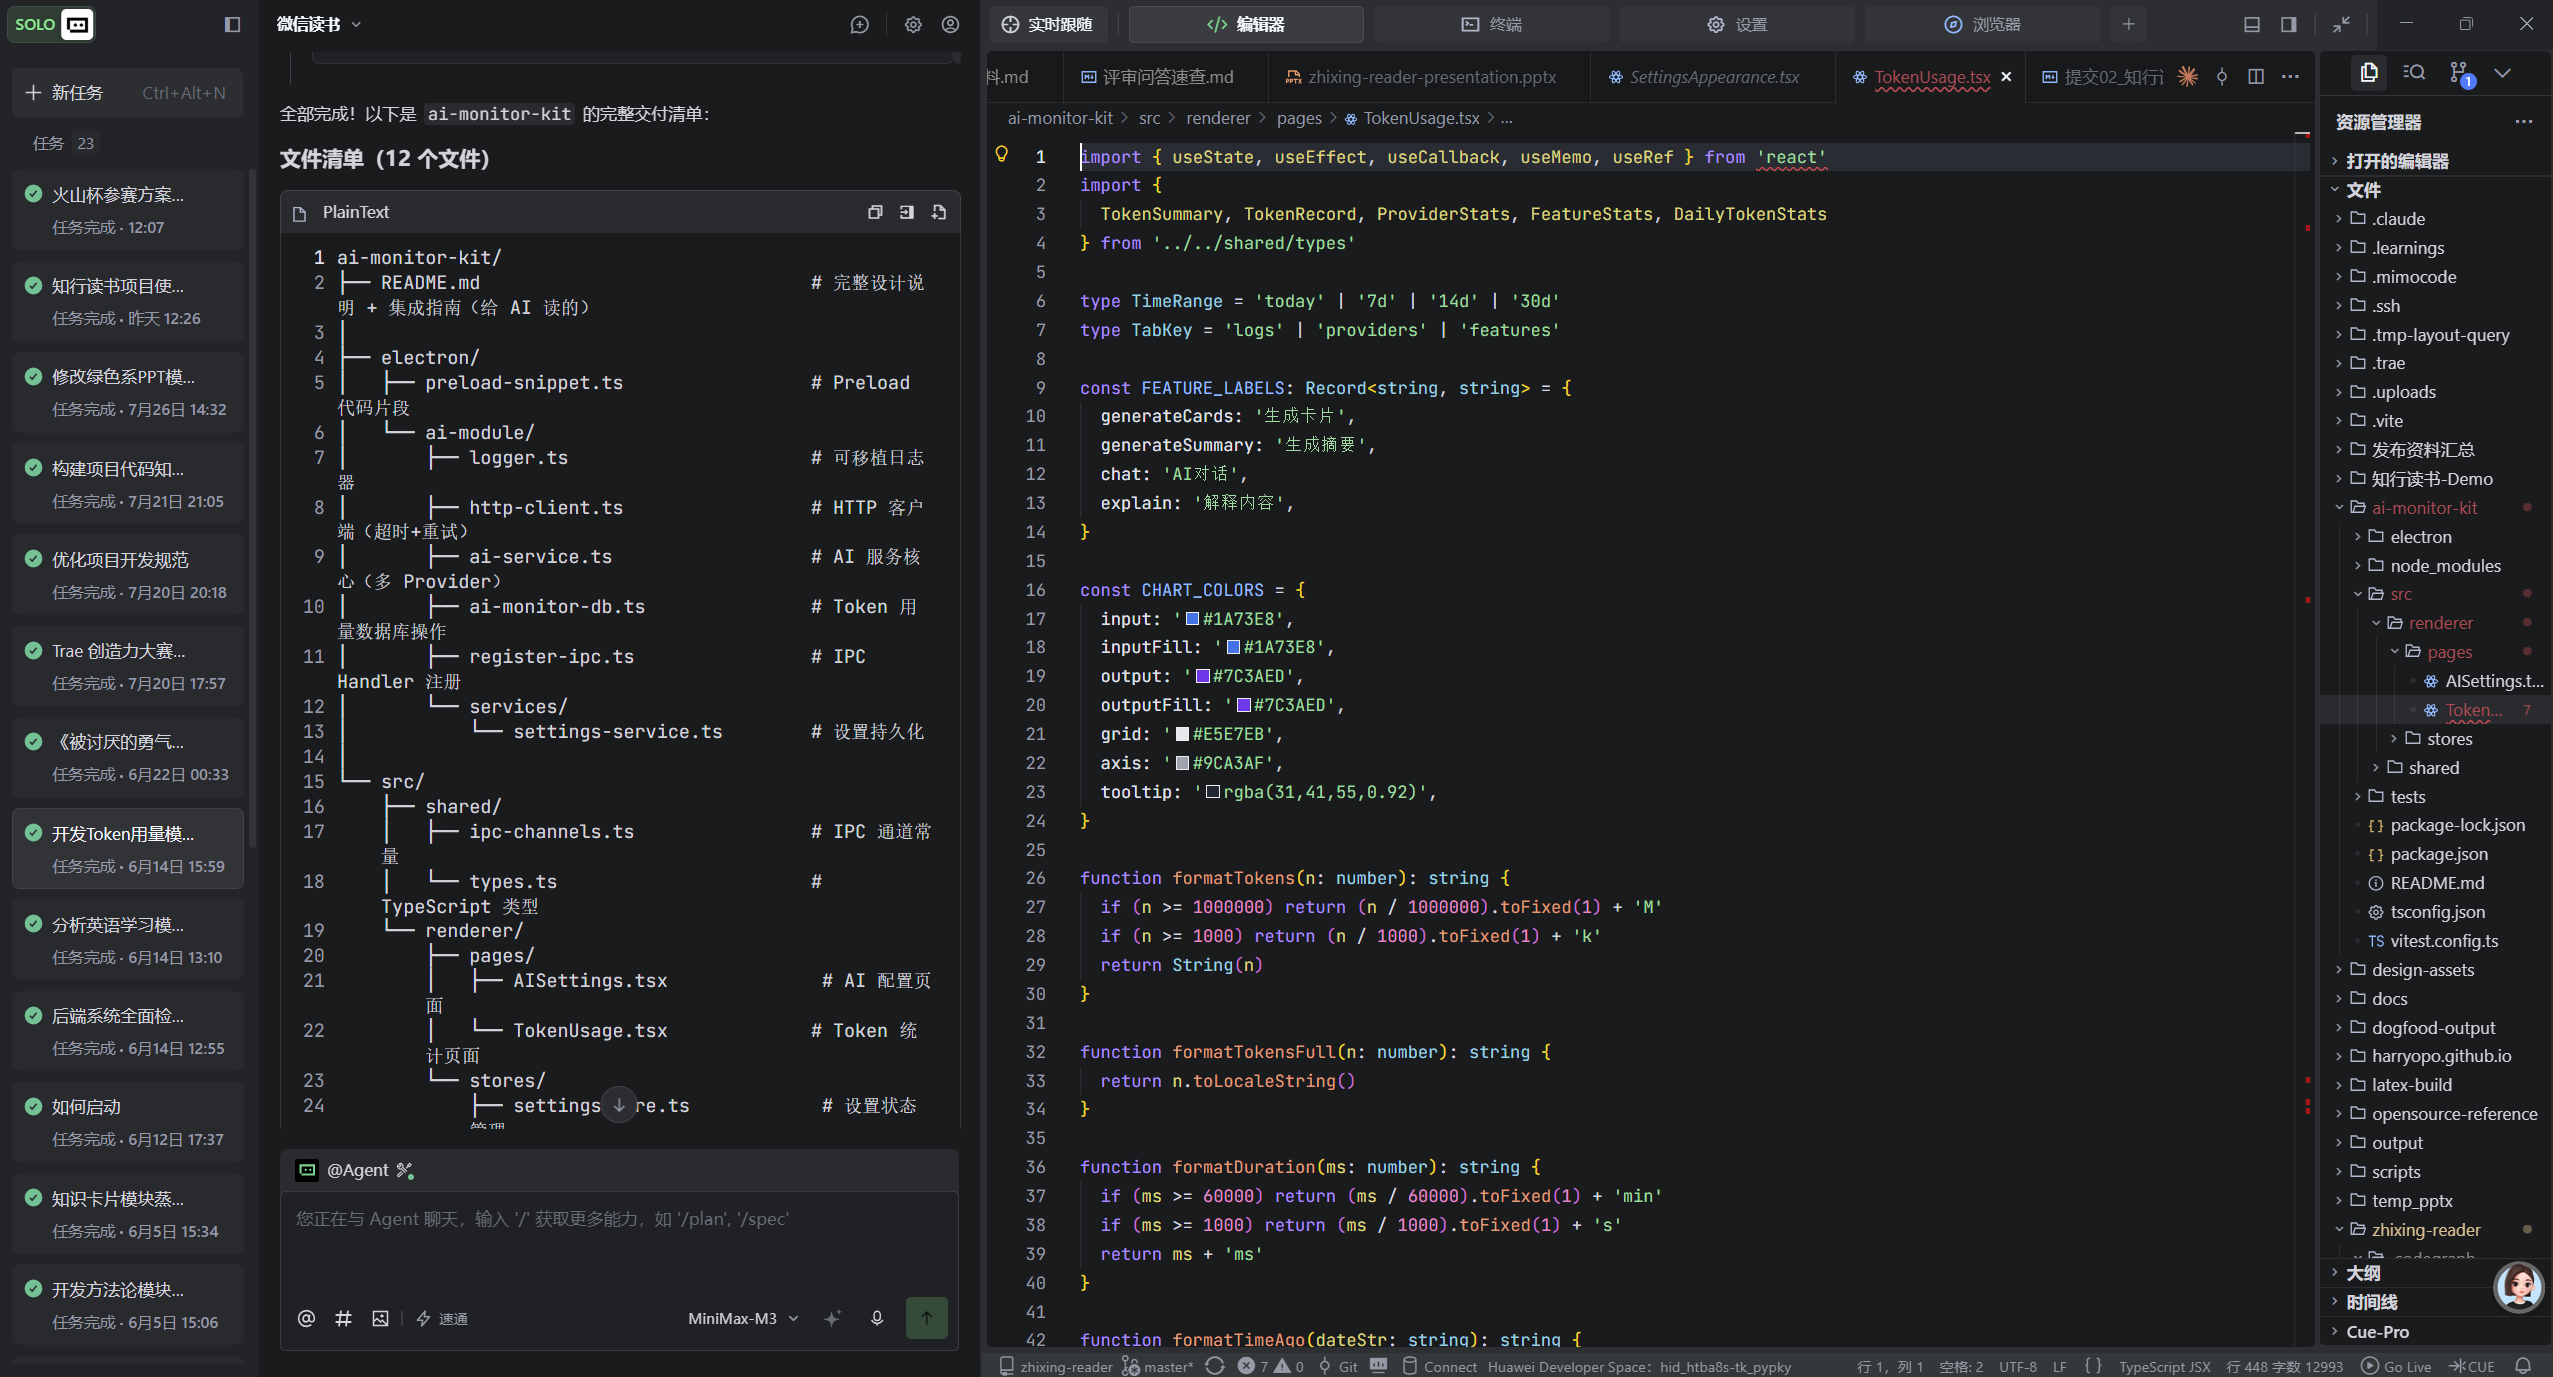
\includegraphics[width=0.48\textwidth]{figures/img_009.png}\hfill
    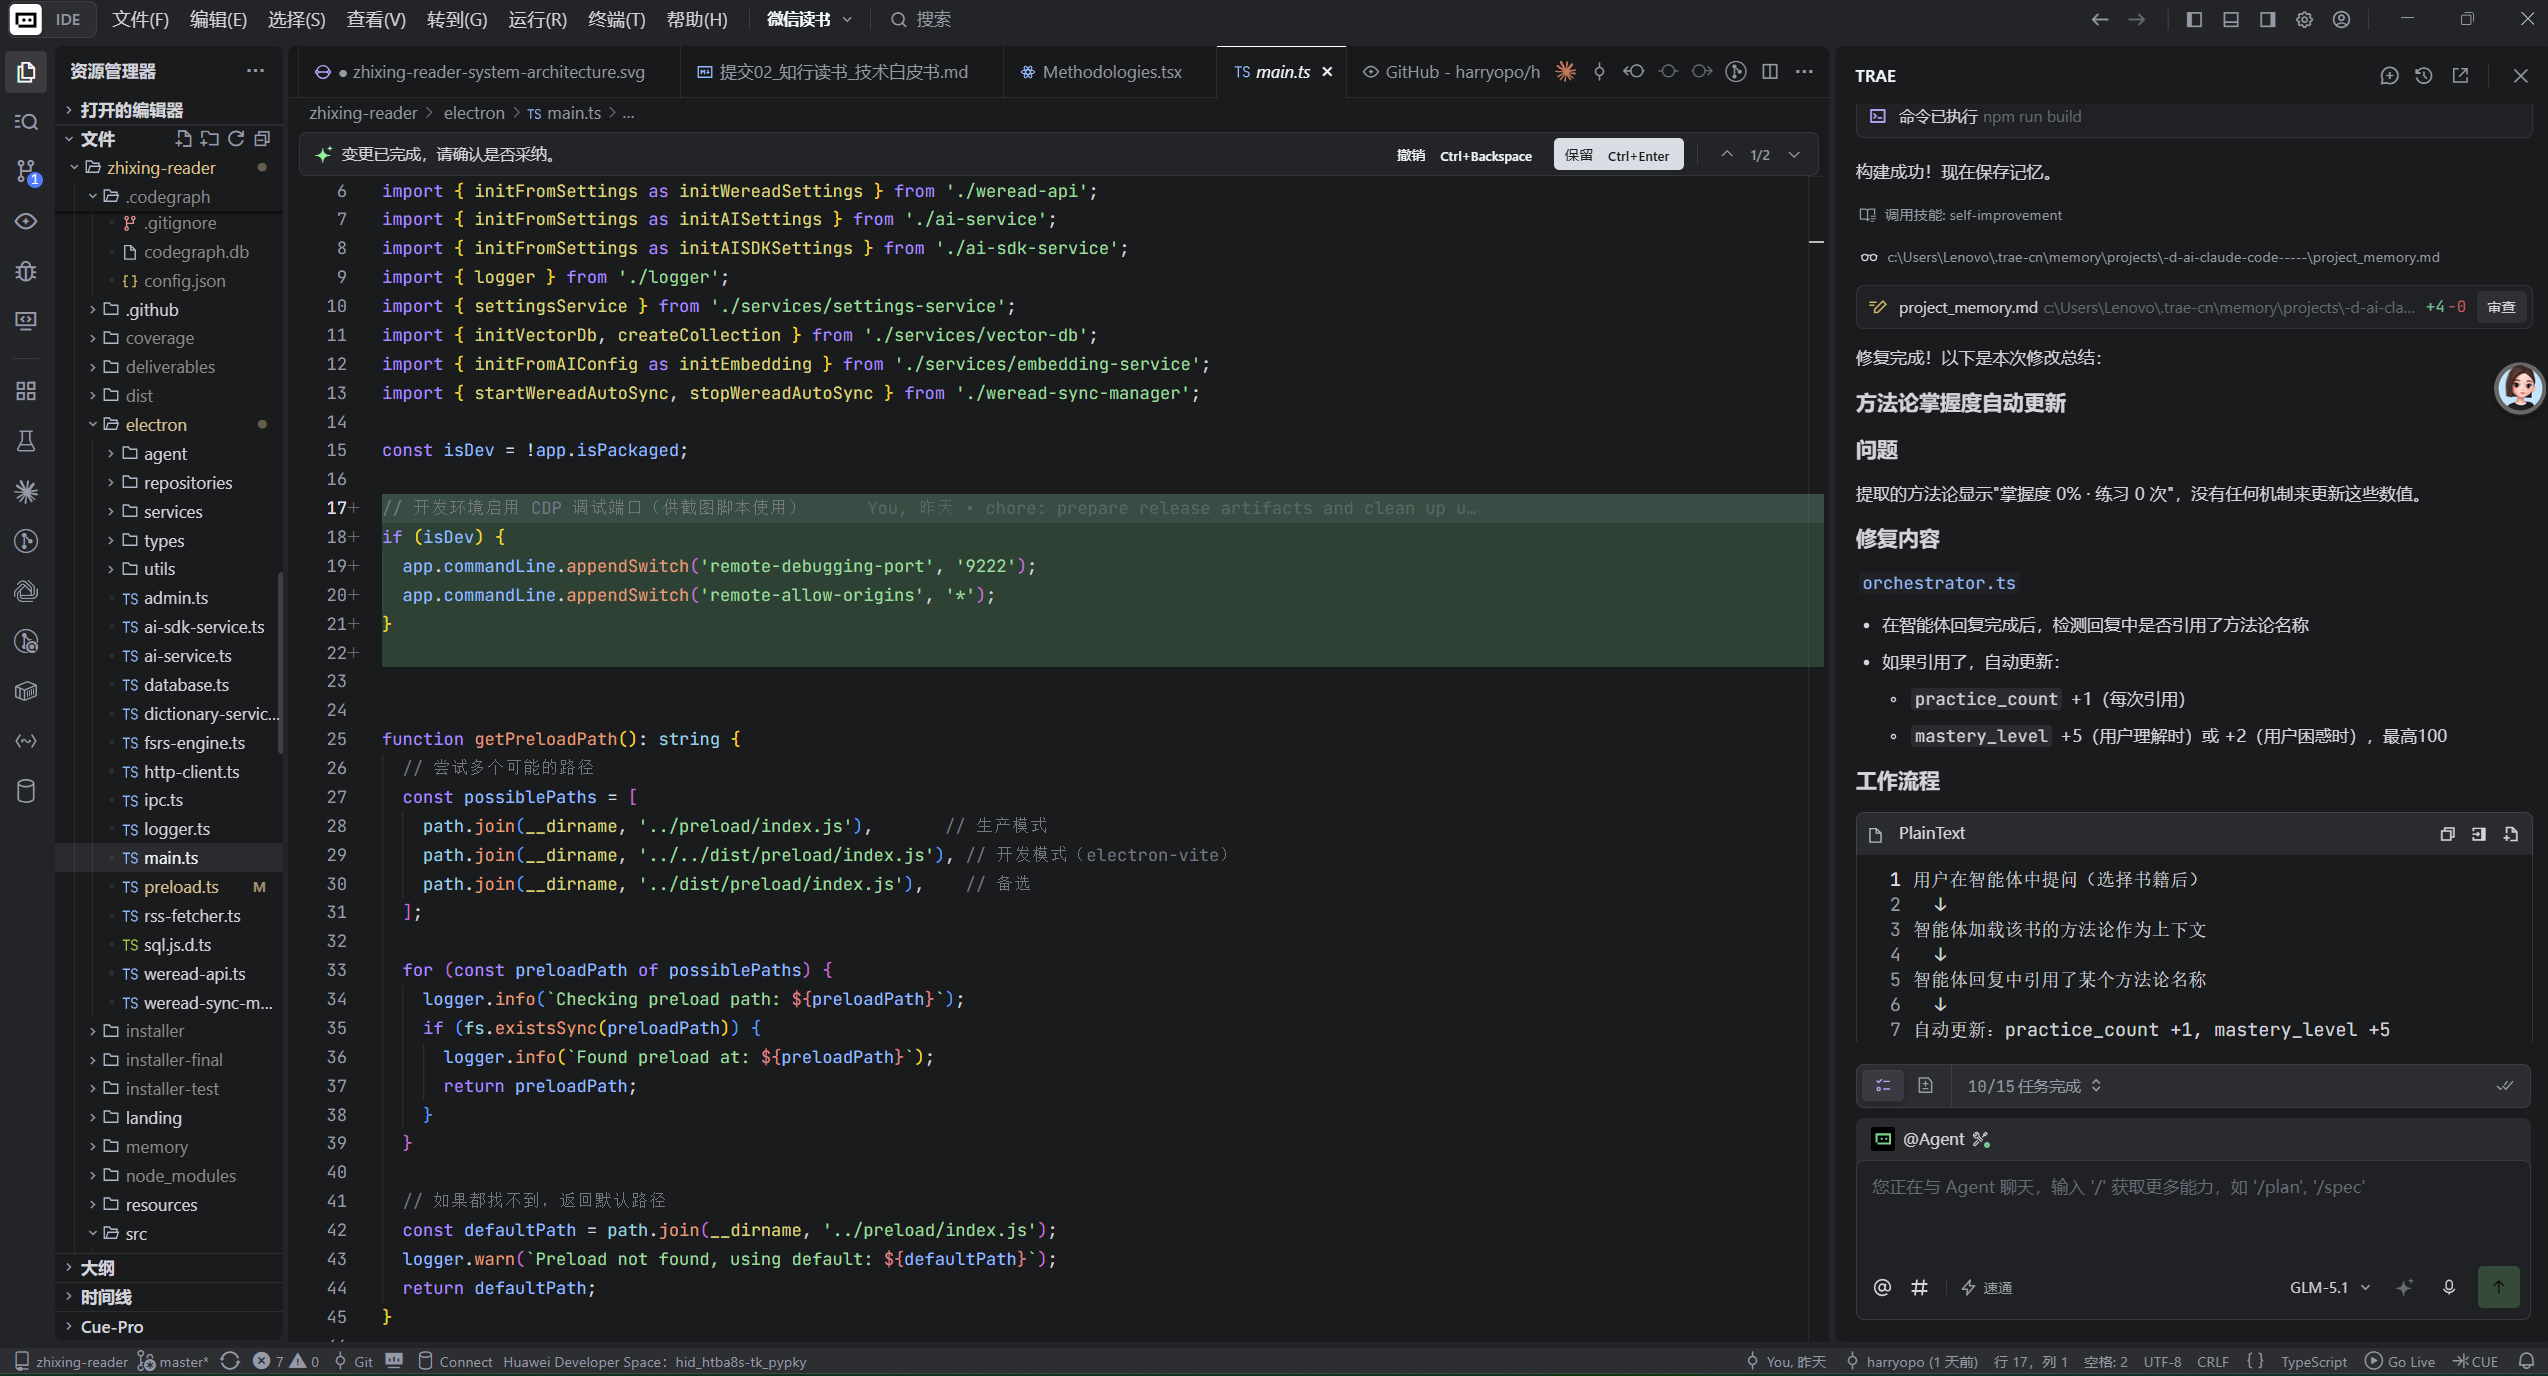
\includegraphics[width=0.48\textwidth]{figures/img_010.png}\\[6pt]
    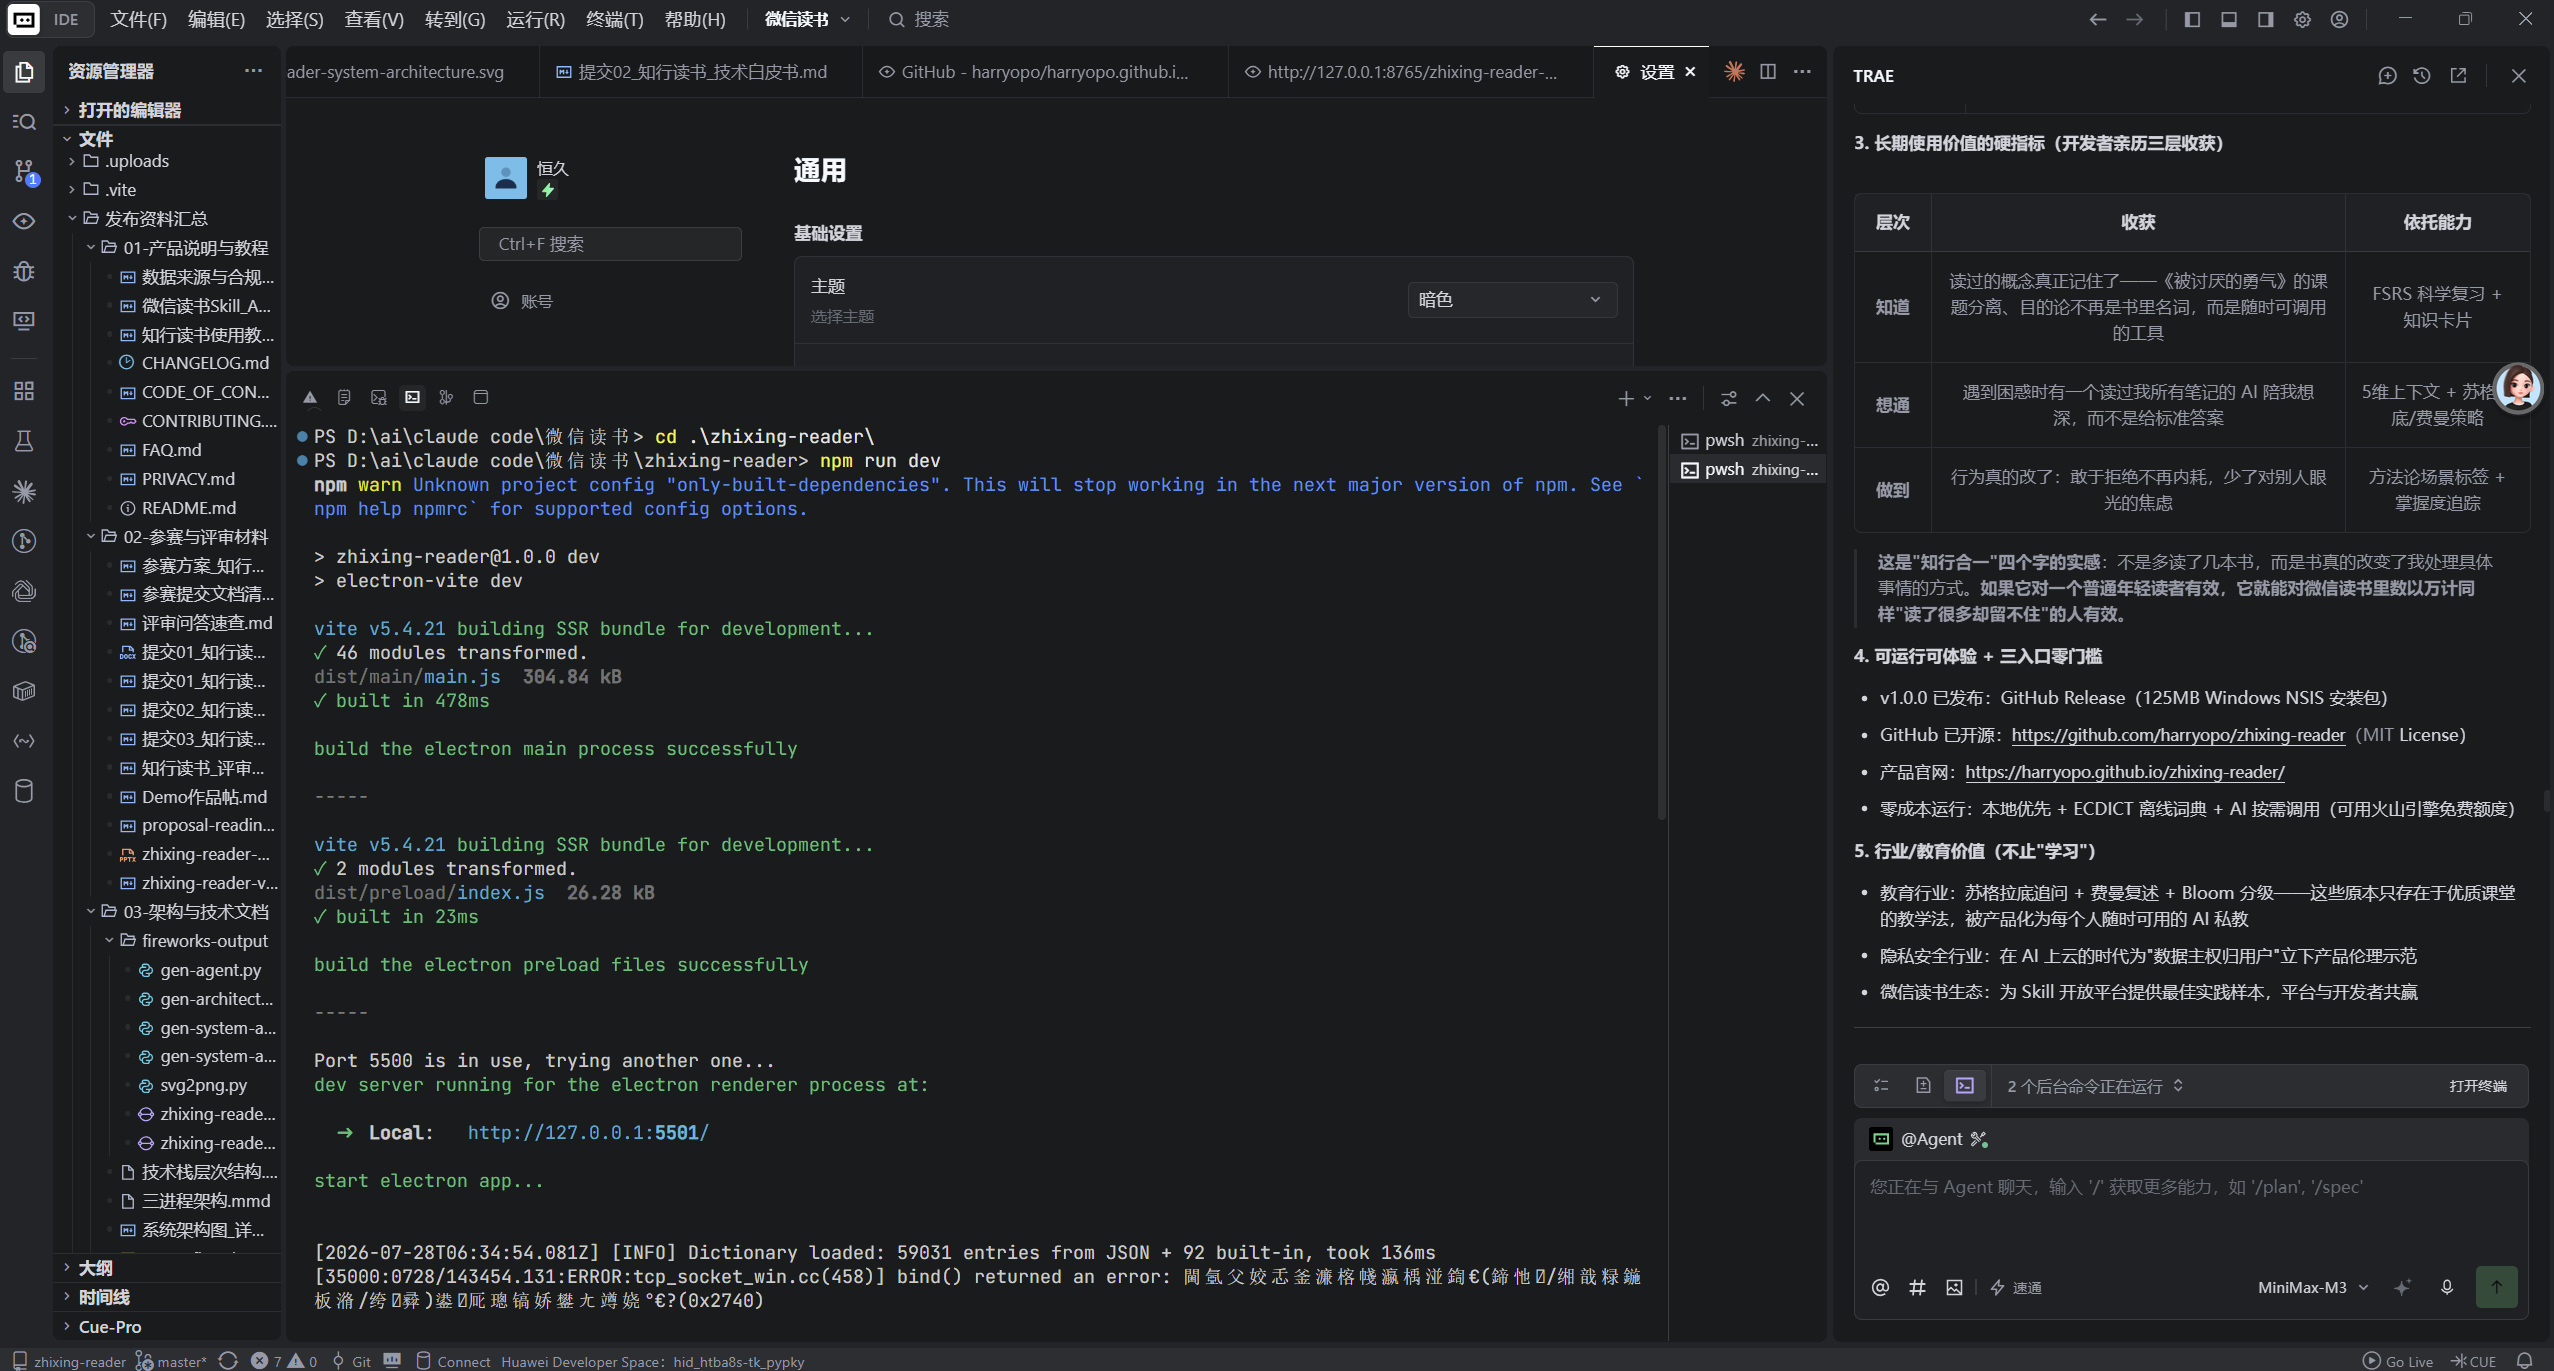
\includegraphics[width=0.48\textwidth]{figures/img_011.png}
    \caption{Trae IDE 使用截图（3 张）}
    \label{fig:trae-ide-2}
\end{figure}

\subhead{Trae work}
\begin{figure}[htbp]
    \centering
    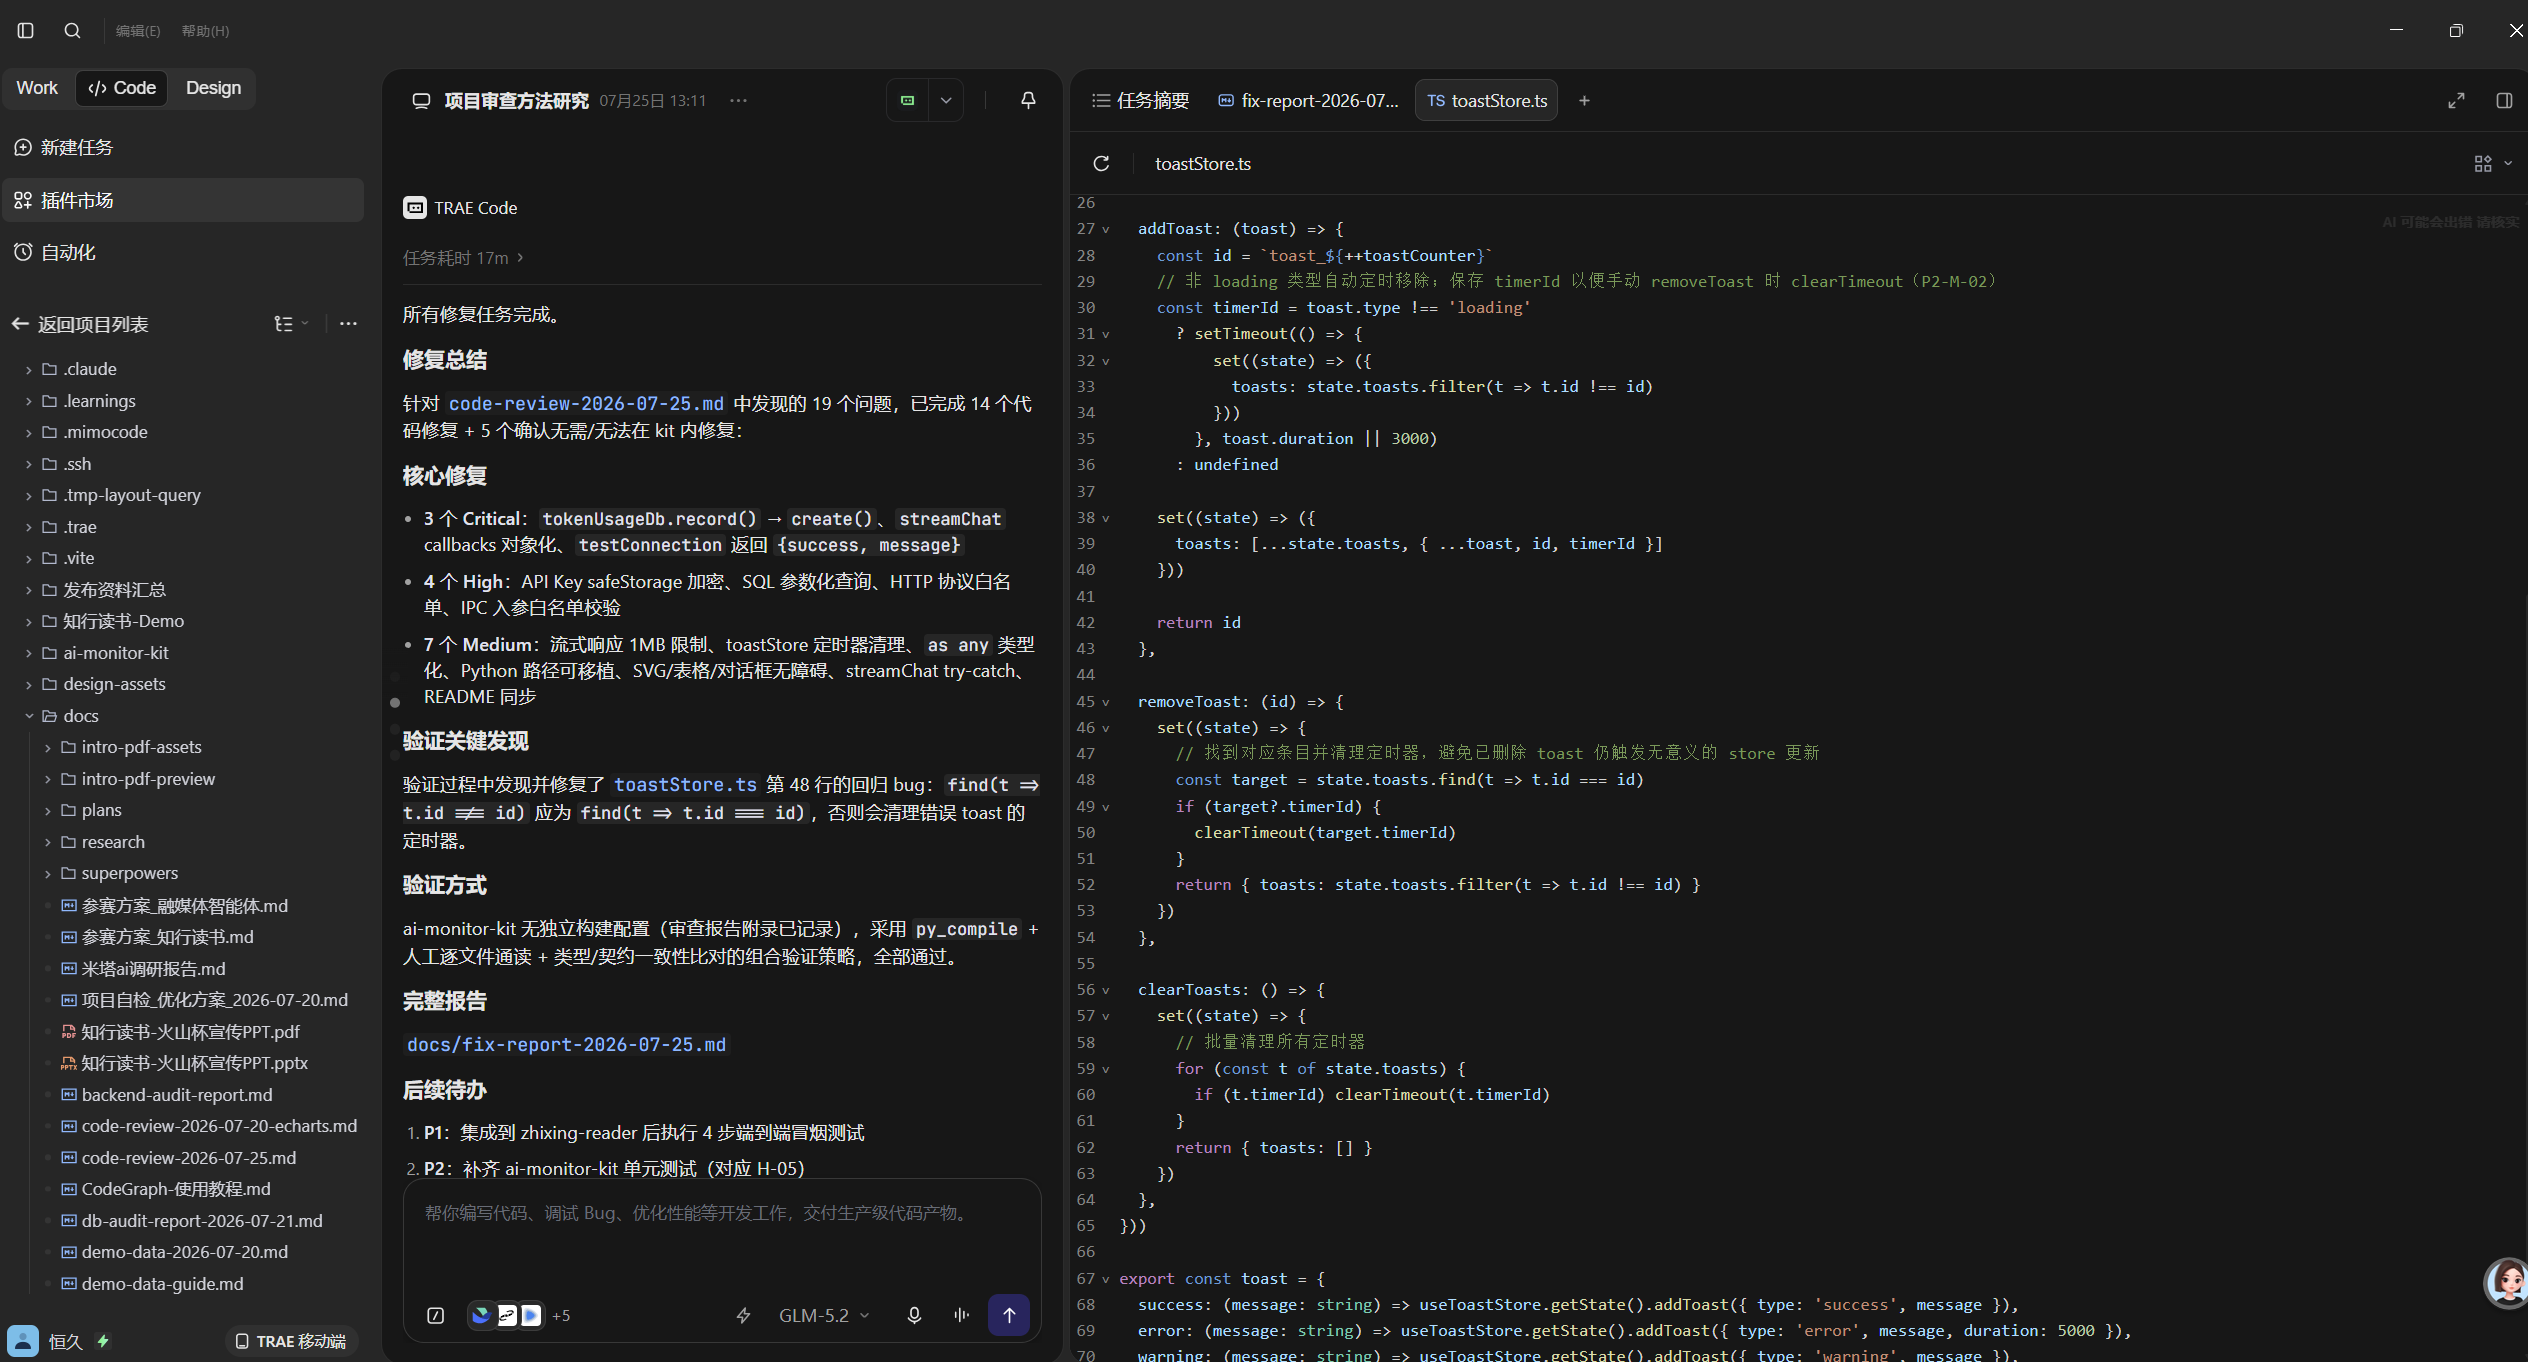
\includegraphics[width=0.48\textwidth]{figures/img_012.png}\hfill
    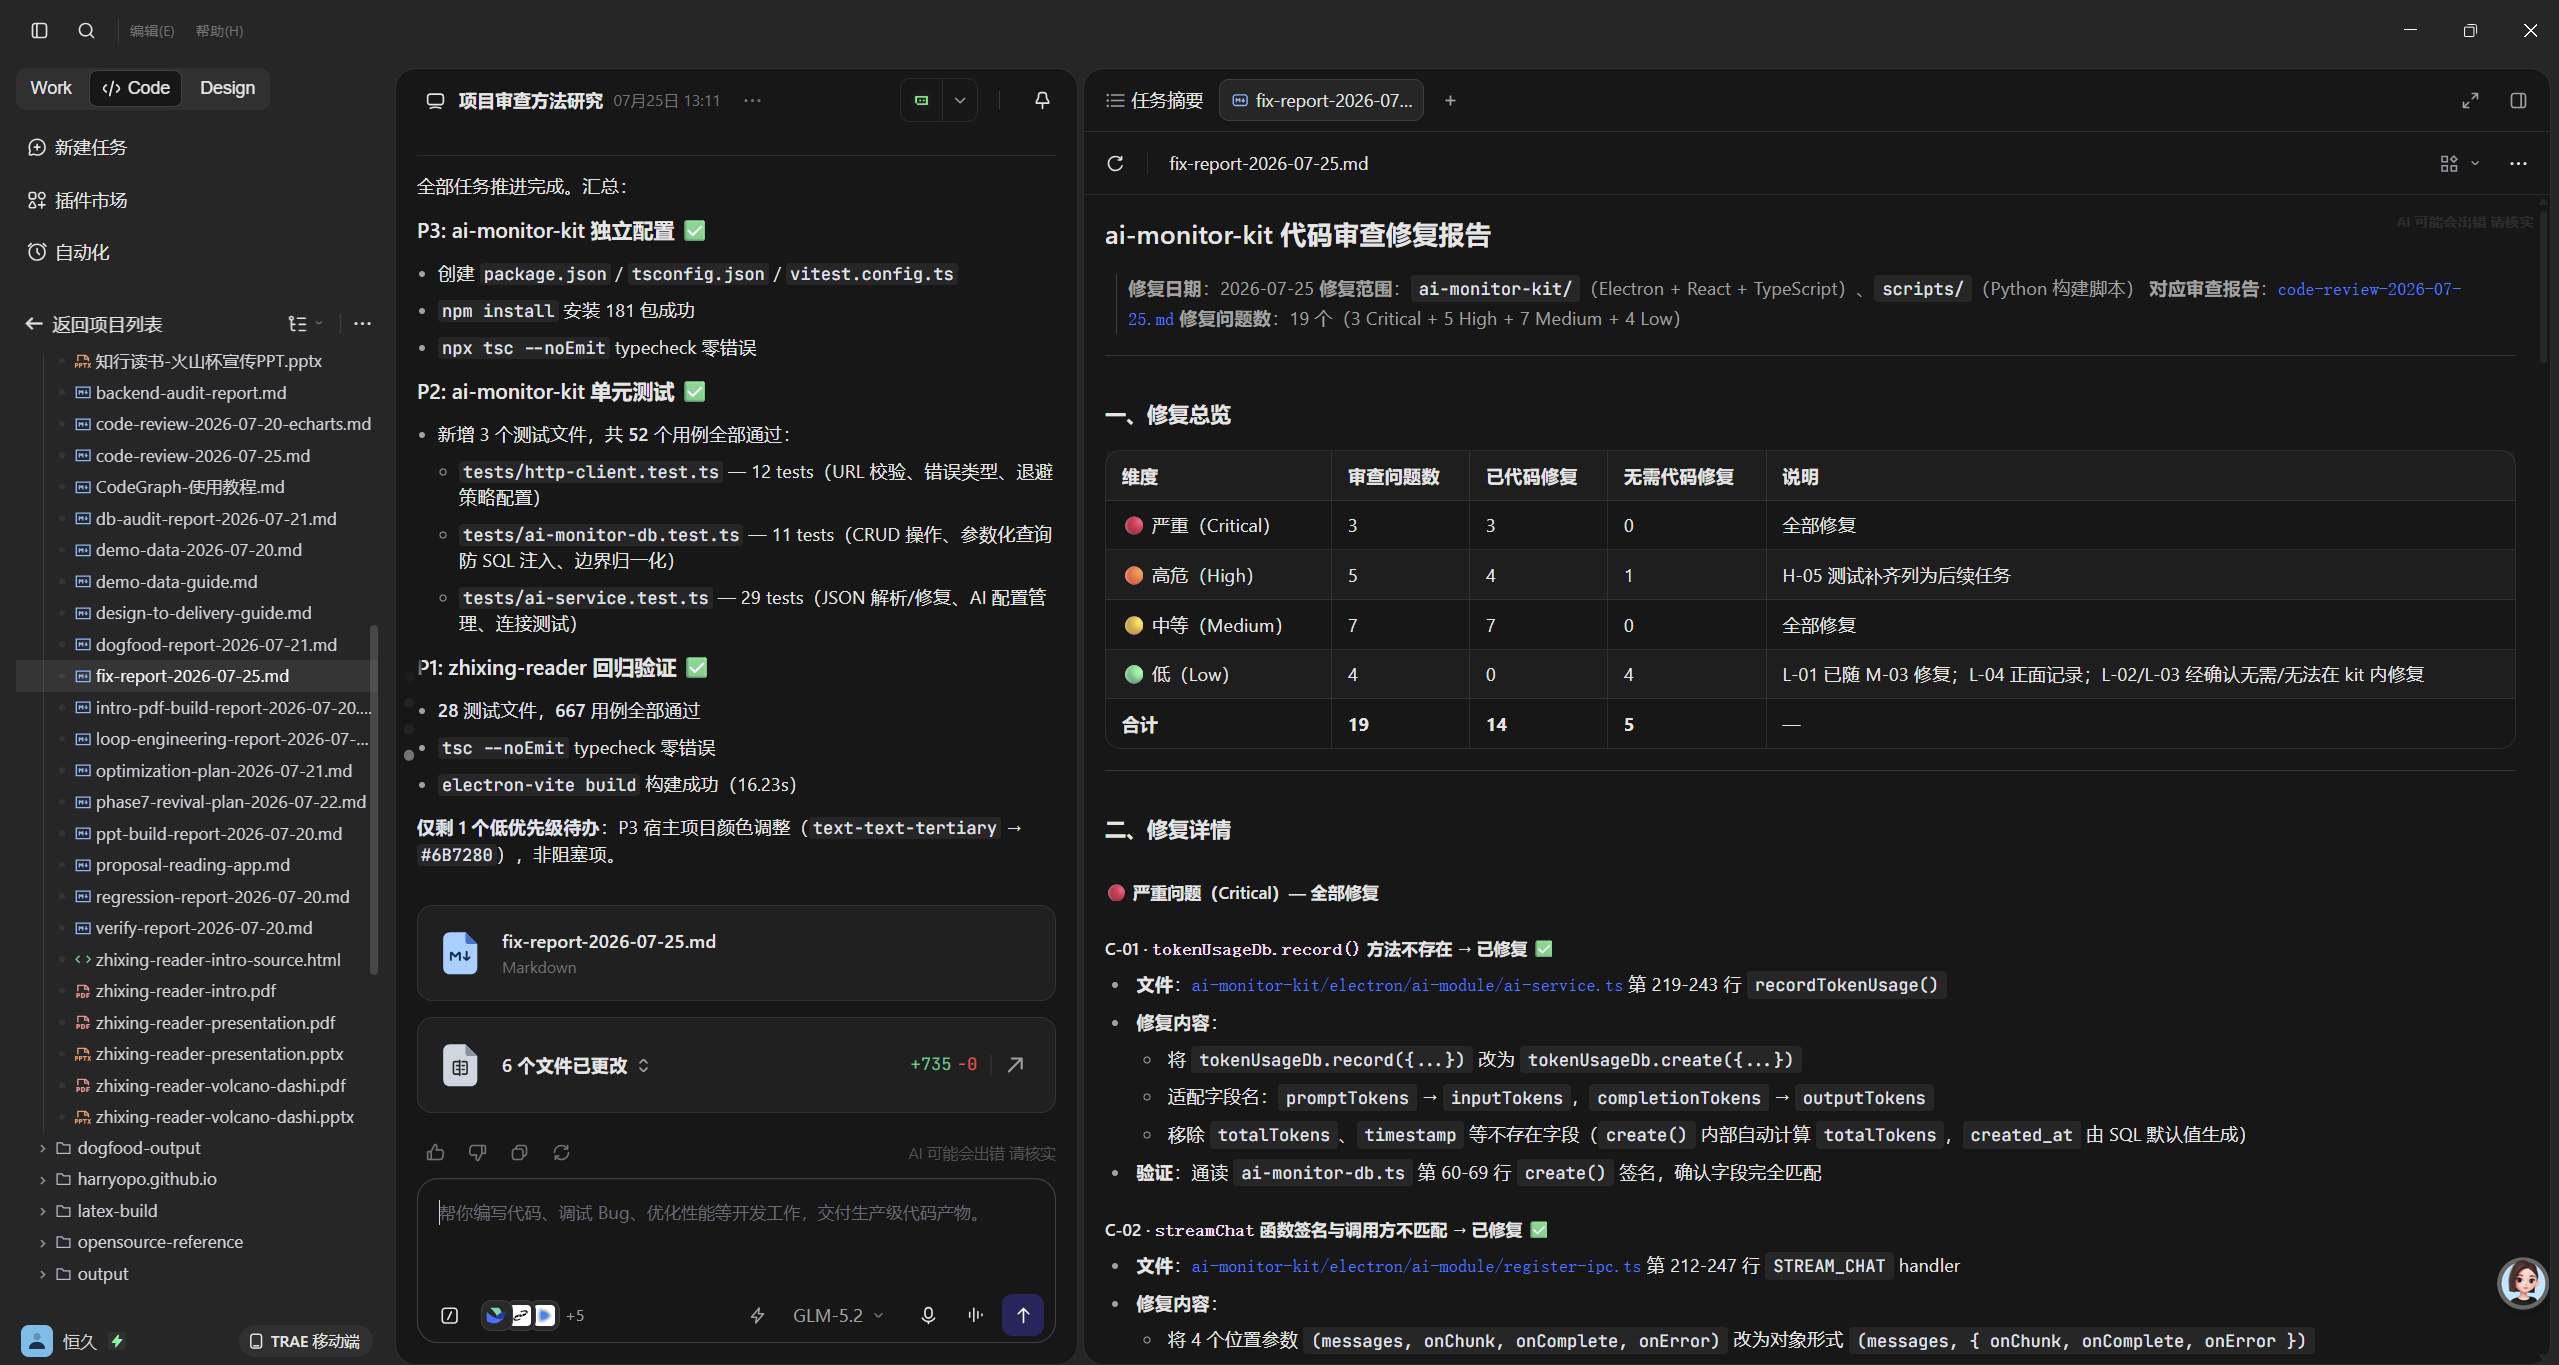
\includegraphics[width=0.48\textwidth]{figures/img_013.png}
    \caption{Trae work 使用截图}
    \label{fig:trae-work}
\end{figure}

\subhead{Trae Design}
\begin{figure}[htbp]
    \centering
    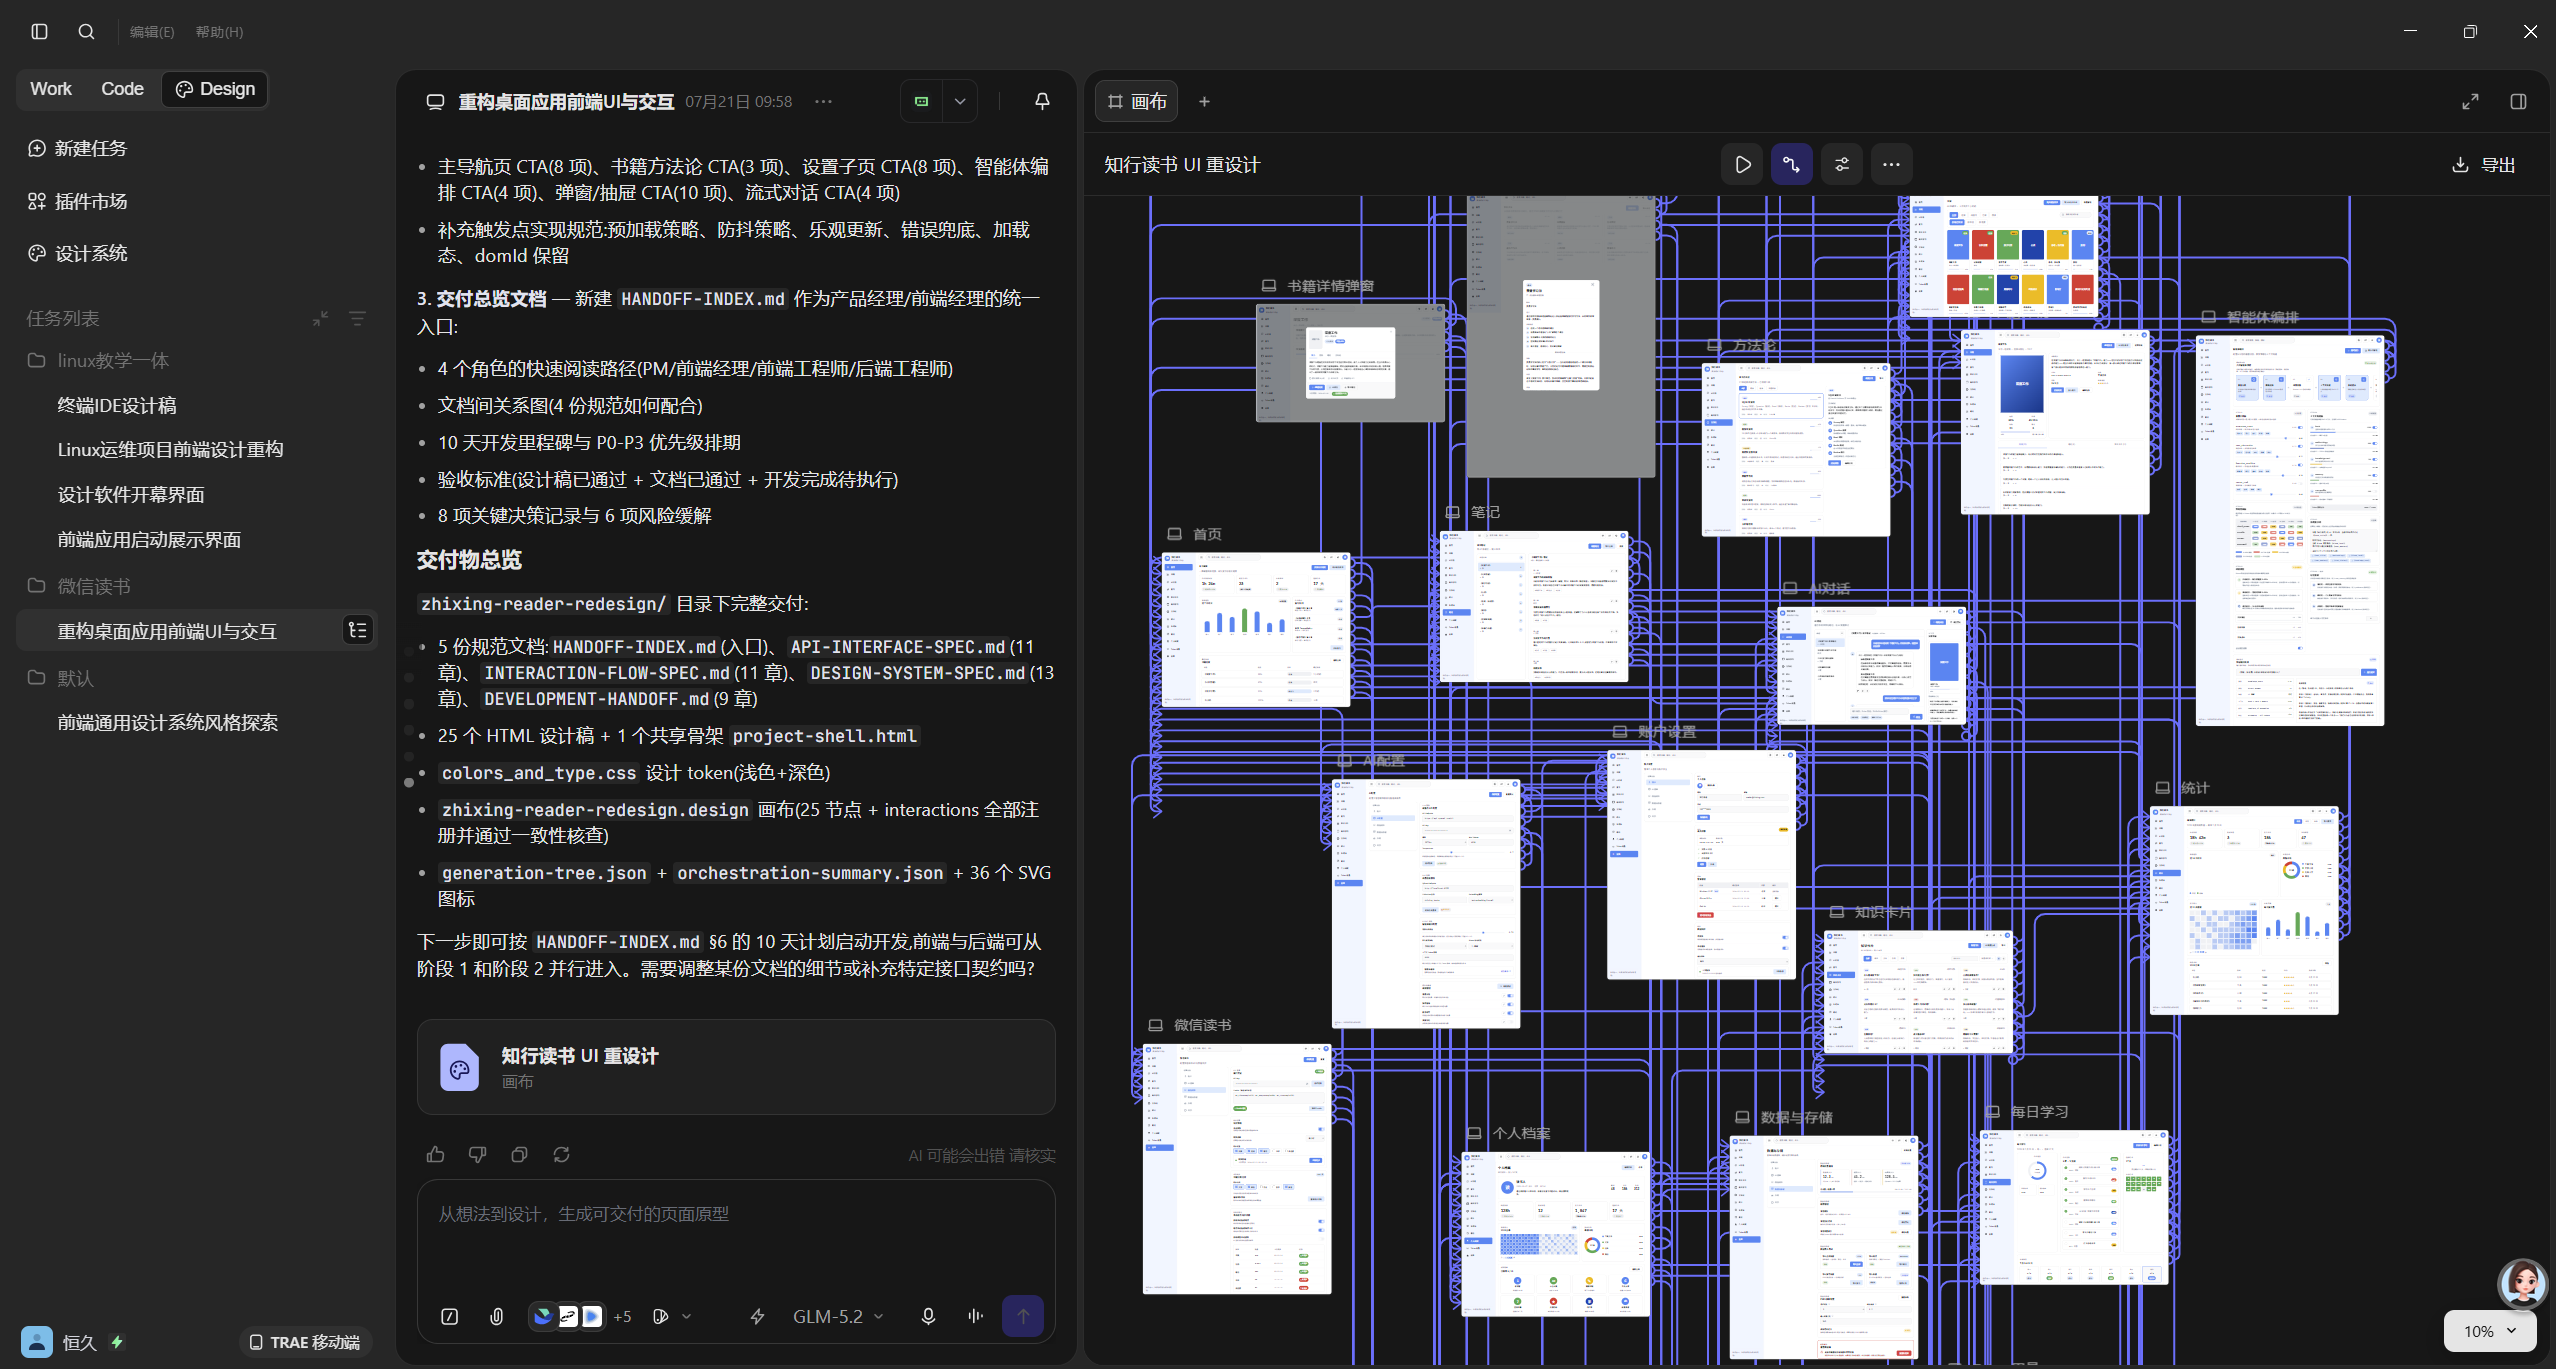
\includegraphics[width=0.48\textwidth]{figures/img_014.png}
    \caption{Trae Design 使用截图}
    \label{fig:trae-design}
\end{figure}

\subhead{部分 Agent ID 样例}
% 风格提示：用 verbatim 或 lstlisting 让 ID 保持原貌
\begin{lstlisting}[style={plainstyle}, caption={Trae Agent 会话 ID 样例}]
.1241824064444384:db4b85dac6c078b3bbb8ff06727b5588_..._2026/7/21 21:03:48
.1241824064444384:972f19dc2f83370d61b0d3d6ceed6e51_..._2026/7/27 12:13:13
\end{lstlisting}

\subsection{使用经验总结}
{占位}我开发项目时，采用"循环工程子 Agent 开发模式"——每个任务由独立的 AI subagent 实施，经 spec 合规审查 + 7 维代码质量审查双门禁通过才进入下一任务，全程沉淀可追溯。这套 AI 协作工程化流程，本身就是对"AI 时代软件工程"的一次完整探索。
\fi

\ifshowthoughts
\section{个人想法}
% 风格提示：完全第一人称感性叙述，可举 1 个具体例子说明产品的"用户价值"
{占位}我自己到底得到了什么？以下是我作为第一个用户的真实自述，也是我最想对评委说的一段话——它回答"这个产品到底能干什么"。

{占位}我最大的感受，是第一次真正与一个"懂我笔记"的 AI 对话。它知道我在哪本书的哪一页划了线，知道我反复关注的是什么主题。问它问题时，它不是给我一段百科全书式的泛泛而谈，而是引用我自己划过的那句话、接着我自己的思考往下追问。

{占位}一个具体的例子：读《XXX》时的真实改变（300-500 字故事性叙述，遵循"以前的我 → 阅读过程 → 现在的我"叙事三段）。
\fi

\ifshowcompetitors
\section{与竞品的差异化}
% 风格提示：5-7 行对比，每行"竞品名 + 它是什么 + 你的差异"
\begin{table}[htbp]
\centering
\begin{tabularx}{\textwidth}{>{\bfseries}l X X}
\toprule
\textbf{竞品} & \textbf{它是什么} & \textbf{本作品的差异} \\
\midrule
竞品 A & 平台型 & 我们是它的"第二大脑"——互补而非竞争 \\
竞品 B & 工具型 & 同一算法，但卡片自动生成，零手工录入 \\
竞品 C & 笔记型 & 数据自动流入，无需手动迁移 \\
竞品 D & 通用 AI & 我们的 AI 读过你读的书，带教学策略 \\
\bottomrule
\end{tabularx}
\caption{与主要竞品的差异分析}
\label{tab:competitors}
\end{table}

\subhead{护城河}三重组合（开放平台 × 间隔重复 × 教学策略 Agent），目前没有第二个产品同时做到。
\fi

\ifshowreviewdetail
\section{评审标准对标}
\label{sec:review}
\begin{table}[htbp]
\centering
\begin{tabularx}{\textwidth}{>{\bfseries}X >{\bfseries}X}
\toprule
\textbf{创新性与创意度（20\%）} & \textbf{技术实现与复杂度（30\%）} \\
\midrule
{占位}为什么是这个智能体？跨学科融合的差异化 & {占位}它是怎么跑起来的？N 大创新点 + N 行代码 \\
\bottomrule
\\
\textbf{实用价值与落地性（30\%）} & \textbf{用户体验与交互设计（20\%）} \\
\midrule
{占位}它好用吗？真实使用数据 + 三入口体验 & {占位}用起来顺手吗？设计系统 + 性能体验 \\
\bottomrule
\end{tabularx}
\caption{四大评审维度对标（按权重分两栏对比）}
\label{tab:review-detail}
\end{table}

\begin{table}[htbp]
\centering
\begin{tabularx}{\textwidth}{>{\bfseries}l X}
\toprule
\textbf{创新点} & \textbf{评分依据} \\
\midrule
创新点 1 & 行业首创，自动引用书中方法论 + 掌握度更新 \\
创新点 2 & 预算制懒加载 + fail-soft，Token 节省 33\%--55\% \\
创新点 3 & ts-fsrs 官方库 + DSR 模型，自动喂卡零手工 \\
创新点 4 & 数据全本地 + AI 云端热切换，数据主权还给用户 \\
创新点 5 & 13.6MB JSON 离线词典，悬停查词毫秒响应 \\
\bottomrule
\end{tabularx}
\caption{5 大创新点对应评分依据}
\label{tab:innovation}
\end{table}

\begin{table}[htbp]
\centering
\begin{tabularx}{\textwidth}{>{\bfseries}l X}
\toprule
\textbf{技术亮点} & \textbf{说明} \\
\midrule
架构亮点 1 & {占位}三进程 + 沙箱最严安全模型 \\
架构亮点 2 & {占位}N,000+ 行 TS strict + N 测试 + 质量门禁 \\
架构亮点 3 & {占位}智能体编排 N 步流水线 + 教学策略 \\
\bottomrule
\end{tabularx}
\caption{技术亮点详表}
\label{tab:tech-highlight}
\end{table}

\begin{table}[htbp]
\centering
\begin{tabularx}{\textwidth}{>{\bfseries}l X}
\toprule
\textbf{落地优势} & \textbf{说明} \\
\midrule
真实用户 & 开发者本人即核心用户，真实使用 N 天 \\
真实场景 & 阅读 → 笔记 → 复习 → 应用 全闭环 \\
可运行可体验 & 已发布 v1.0.0，三入口（安装包/源码/官网） \\
零成本 & 本地优先 + 离线词典 + 免费额度可用 \\
开源可持续 & MIT + 全套社区文档 \\
\bottomrule
\end{tabularx}
\caption{落地优势详表}
\label{tab:landing}
\end{table}
\fi

\ifshowvalue
\section{应用价值}
\subhead{用户价值}把每本书的阅读投入转化为长期认知资产——划线自动变卡片、卡片科学调度复习、AI 私教检验理解、方法论指导实践。

\subhead{教育价值}苏格拉底追问 + 费曼复述 + Bloom 分级这些原本只存在于优质课堂的教学法，被产品化为每个人随时可用的 AI 私教。

\subhead{商业前景}（宗旨还是开源）
\begin{itemize}
    \item 知识服务：方法论库、学习路径规划
    \item 生态位：上游平台海量注册用户中的深度学习者是天然种子盘
\end{itemize}

\subhead{社会价值}
\begin{itemize}
    \item 把"读过"变成"学会"，提升全民深度阅读的实际回报
    \item 用本地优先架构示范"数据主权归用户"的产品伦理
    \item 为开放生态提供最佳实践样本
\end{itemize}
\fi

\ifshowfuture
\section{未来规划}
\begin{table}[htbp]
\centering
\begin{tabularx}{\textwidth}{>{\bfseries}l X}
\toprule
\textbf{阶段} & \textbf{计划} \\
\midrule
短期（3--6 月） & 持续迭代优化，修复 bug，扩大开源生态，多宣传；尝试导入更多数据源；社区方法论分享；macOS 端适配 \\
中期（6--12 月） & 知识图谱可视化、协作学习小组、MCP 开发 \\
长期（1--2 年） & 插件生态与开放 API、个性化模型微调、企业团队知识管理版 \\
\bottomrule
\end{tabularx}
\caption{未来规划分阶段计划}
\label{tab:future}
\end{table}
\fi

% =====================================================================
% 第 4 章：数据来源与合规说明
% =====================================================================
\ifshowappendix
\chapter{数据来源与合规说明}

\section{数据来源}
\begin{table}[htbp]
\centering
\begin{tabularx}{\textwidth}{>{\bfseries}l X X X}
\toprule
\textbf{数据类别} & \textbf{说明} & \textbf{存储位置} & \textbf{是否上传} \\
\midrule
用户主动输入 & 聊天消息 / 笔记 / 复习评分 & 本地 SQLite & 否 \\
上游平台同步 & 书架 / 划线 / 笔记 / 书评 & 本地 SQLite & 否 \\
AI 服务请求 & 对话上下文 / 模型响应 & AI 服务商 & 是（按需） \\
系统生成数据 & 知识卡 / 方法论 / 记忆 & 本地 SQLite & 否 \\
\bottomrule
\end{tabularx}
\caption{四类核心数据矩阵}
\label{tab:data-source}
\end{table}

\section{合规性声明}

\subhead{开放平台 API 使用合规}
\begin{itemize}
    \item 遵循开放平台服务条款
    \item 仅用于个人学习和非商业用途
    \item 不爬取、不存储用户隐私信息
    \item 尊重用户知识产权
    \item 用户自主申请 API Key 并授权
\end{itemize}

\subhead{AI 服务使用合规}
\begin{itemize}
    \item 遵循各 AI 服务商的使用条款（火山引擎 / DeepSeek / OpenAI / Anthropic）
    \item 不生成违法、有害内容
    \item 用户对 AI 生成内容负责
    \item 请求直连服务商，不经过任何中转服务器
\end{itemize}

\subhead{数据安全合规}
\begin{itemize}
    \item 符合《个人信息保护法》要求
    \item 明确告知用户数据用途
    \item 提供数据导出和删除功能
    \item 不向第三方共享用户数据
    \item 开源协议遵循（MIT License）
\end{itemize}

\subhead{开源声明}
本项目以 MIT License 开源，源代码托管于 GitHub（org/repo）。所有第三方组件的版权与商标归其原作者所有。

% =====================================================================
% 第 5 章：使用教程与常见问题解答
% =====================================================================
\chapter{使用教程与常见问题解答}

\section{使用教程}

\subhead{系统要求}
\begin{itemize}
    \item 操作系统：Windows 10 / 11（64 位）
    \item 内存：≥ 4GB RAM（推荐 8GB）
    \item 硬盘：≥ 500MB 可用空间
    \item 网络：仅同步 + AI 对话需要联网（其他功能可离线）
\end{itemize}

\subhead{下载与安装}
\begin{enumerate}
    \item 访问 GitHub Releases 页面
    \item 下载最新的安装包
    \item 双击安装包，按向导完成安装
    \item 启动应用，进入主界面
\end{enumerate}

\subhead{首次启动}
\begin{enumerate}
    \item 首次启动会创建本地数据目录
    \item 建议在「设置 → AI 配置」中填入你的 AI 服务商 API Key
    \item 在「设置 → 上游平台」中填入 API Key，连接你的账号
\end{enumerate}

\ifshowfaq
\section{常见问题 FAQ}
% 风格提示：每条 Q 用加粗 Q 前缀，答用 答：前缀

% --- 通用 FAQ（所有项目类型通用） ---
\subhead{Q1：在哪里下载安装包？}
答：从 GitHub Releases 页面下载最新的安装包，双击安装即可。

\subhead{Q2：为什么安装包这么大？}
答：主要来自桌面运行时 + SQLite WASM 引擎 + 图表库，这是桌面应用的正常体积。

\subhead{Q3：支持 macOS / Linux 吗？}
答：当前仅提供 Windows 安装包。macOS / Linux 需要克隆仓库后自行构建。

\subhead{Q4：如何更新到新版本？}
答：应用会通过 GitHub Releases API 自动检查更新并提示；也可以手动到 Releases 页面下载新版安装包覆盖安装，本地数据不会丢失。

\subhead{Q5：我的数据存在哪里？会上传吗？}
答：所有数据都存储在本地 SQLite 数据库，不上传任何服务器。应用不包含分析、追踪或广告 SDK。

\subhead{Q6：如何备份数据？}
答：直接复制本地数据库文件即可完整备份；也可以在应用内使用导出功能。

\subhead{Q7：支持离线使用吗？}
答：支持。除同步和 AI 对话需要联网外，其余功能均可离线使用。

\subhead{Q8：如何连接上游平台？}
答：进入「设置 → XXX」，填入 API Key，点击「测试连接」，成功后点击「同步」。

\subhead{Q9：同步失败怎么办？}
答：按顺序排查：1) 检查 API Key 是否有效；2) 检查网络连接；3) 是否触发了频率限制（稍后重试）；4) 手动触发。

\subhead{Q10：多久自动同步一次？}
答：默认每 15 分钟自动同步一次，可在设置中调整。

% --- 软件/AI 项目 FAQ（可选） ---
\ifx\projectType AISOFTWARE
\subhead{Q11：AI 对话需要自己的 API Key 吗？}
答：需要。进入「设置 → AI 配置」填入你的 AI 服务商 API Key。

\subhead{Q12：什么是「深度思考」模式？}
答：开启后会展示 AI 的推理过程，适合需要看推理链的深度学习场景。

\subhead{Q13：AI 对话和普通聊天机器人有什么区别？}
答：本作品的智能体会根据你的意图自动切换教学策略：直接回答 / 苏格拉底追问 / 费曼复述。

\subhead{Q14：一次对话消耗多少 Token？}
答：约 500--2000 tokens（取决于上下文和回复长度）。可在用量监控页查看详细统计。

\subhead{Q15：复习算法是什么？}
答：采用 FSRS v5 算法，与 Anki 同源，DSR 模型。卡片数据结构与 Anki 兼容。

\subhead{Q16：复习评分怎么选？}
答：1 忘记 / 2 困难 / 3 良好 / 4 简单。算法会根据评分自动调整下次复习时间。

\subhead{Q17：生词本怎么用？}
答：阅读英文内容时选中单词点击「添加到生词本」，系统自动查询释义。
\fi

% --- 硬件项目 FAQ（可选） ---
\ifx\projectType HARDWARE
\subhead{Q11：硬件如何固件升级？}
答：通过 USB 连接电脑，使用官方升级工具即可完成固件升级。

\subhead{Q12：电池续航多久？}
答：正常使用场景下约 N 小时，具体取决于使用模式。

\subhead{Q13：是否支持第三方配件？}
答：支持标准接口，可兼容主流第三方传感器/执行器。
\fi

% --- 通用结尾 FAQ ---
\subhead{Q18：应用启动后白屏 / 打不开怎么办？}
答：1) 完全退出后重新启动；2) 检查杀毒软件是否拦截；3) 重新安装最新版本；4) 在 GitHub Issues 反馈。

\subhead{Q19：如何反馈 Bug 或提功能建议？}
答：到 GitHub Issues 提交，描述清楚：使用版本、操作步骤、预期行为、实际行为（最好附截图）。

\subhead{Q20：如何参与贡献？}
答：阅读 CONTRIBUTING.md 了解开发环境搭建和 PR 流程，提交前确保质量门禁全绿。
\fi

% =====================================================================
% 第 6 章：致谢
% =====================================================================
\chapter{致谢}

{致谢占位}风格提示：感性叙述，第一人称，分 4 段致谢 4 类对象：
(1) 学校和学院——平台与机会
(2) 比赛主办方与技术平台——基础设施与 token 支持
(3) 开放平台——数据底座（如适用）
(4) 开源社区——站在巨人肩膀上

最后用 1 段情怀收尾（如"AI 时代我们要……，但最珍贵的还是人本身"）。

\vspace{1em}
\begin{center}
\itshape ——知之真切笃实处即是行，行之明觉精察处即是知。\\[6pt]
王阳明《传习录》
\end{center}

% =====================================================================
% 可选：参考文献
% =====================================================================
\ifshowbib
\begin{thebibliography}{99}
\bibitem{ref1} {占位}FSRS v5 算法原始论文 / 官方文档
\bibitem{ref2} {占位}Anki 间隔重复算法说明
\bibitem{ref3} {占位}Electron 官方文档
\bibitem{ref4} {占位}微信读书开放平台 API 文档
\bibitem{ref5} {占位}Vectra 向量索引文档
\bibitem{ref6} {占位}MIT License 协议文本
\end{thebibliography}
\fi

% =====================================================================
% 基金信息（如有）
% =====================================================================
\printfunding

\end{document}
